\documentclass[svgnames]{beamer}
\usepackage{graphicx}
\usepackage{textpos}
\usepackage{tikz}
\usepackage[percent]{overpic}
\usepackage{amssymb}% http://ctan.org/pkg/amssymb
\usepackage{pifont}% http://ctan.org/pkg/pifont
\newcommand{\cmark}{\ding{51}}%
\newcommand{\xmark}{\ding{55}}%

\usetheme{Boadilla}
\usecolortheme{dolphin}

\setbeamertemplate{navigation symbols}{}
\setbeamertemplate{itemize items}[default]
\setbeamertemplate{enumerate items}[default]
\setbeamertemplate{blocks}[default]

\graphicspath{{fig/}}

\title[]{Alternative to the two-component ansatz and implications for small collision systems}
\subtitle[Duke U.]{\vspace{0.2 in}} %\includegraphics[scale=0.25]{collision}}
\author[]{} 
\date[\today]{} 

\newcommand{\trento}{T\raisebox{-.5ex}{R}ENTo}
\newcommand{\nch}{N_\text{ch}}

\begin{document}

%%%%%%%%%%%%%%%%%%%
\begin{frame}
\vspace{0 in}
\maketitle

%\begin{textblock*}{\linewidth}(4.5cm,-3.cm)
% \centering 
\includegraphics[scale=0.5]{trento-profile}
%\end{textblock*}

\begin{textblock*}{\linewidth}(0 cm, -0.5 cm)
  \flushleft 
\includegraphics[height=1.2cm]{DukeQCD}
\end{textblock*}

\begin{textblock*}{\linewidth}(0.1 cm, -0.7 cm)
  \flushright 
\includegraphics[height=1.6cm]{Krell}
\end{textblock*}

\begin{textblock*}{\linewidth}(0 cm, 0.8 cm)
  \centering
  \tiny Supported by NNSA Stewardship Science Graduate Fellowship
\end{textblock*}


\begin{textblock*}{\linewidth}(0cm,-2.4cm)
  \centering
  \small
  J.S. Moreland, J.E. Bernhard, S.A. Bass \textbar ~\today \\
  Correlations and Fluctuations in p+A and A+A Collisions \\
  
\end{textblock*}
  
\end{frame}

%%%%%%%%%%%%%%%%%%%%

\begin{frame}{Thinking of initial conditions as a mapping}
  \begin{textblock*}{\linewidth}(-3 cm, -2.5 cm)
    \centering Side view \\
    \vspace{0.1 in} 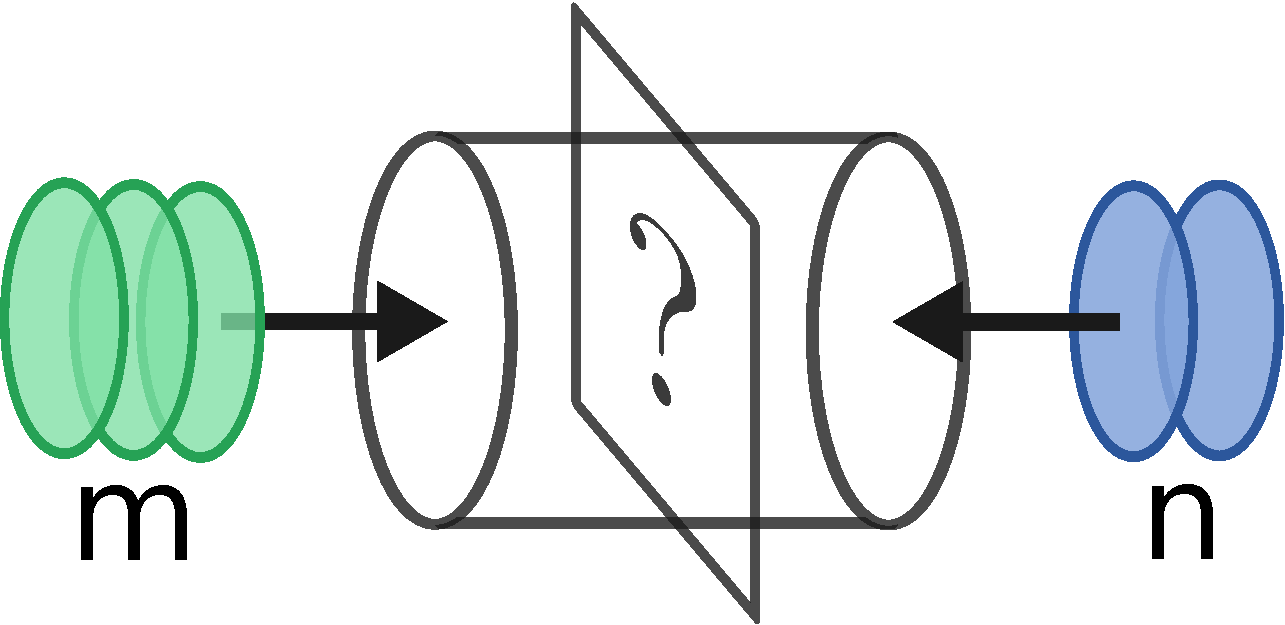
\includegraphics[width=0.35\linewidth]{motivation2}
  \end{textblock*}
 
  \begin{textblock*}{\linewidth}(3 cm, -2.5 cm)
    \centering Beam view \\
    \vspace{0.1 in} 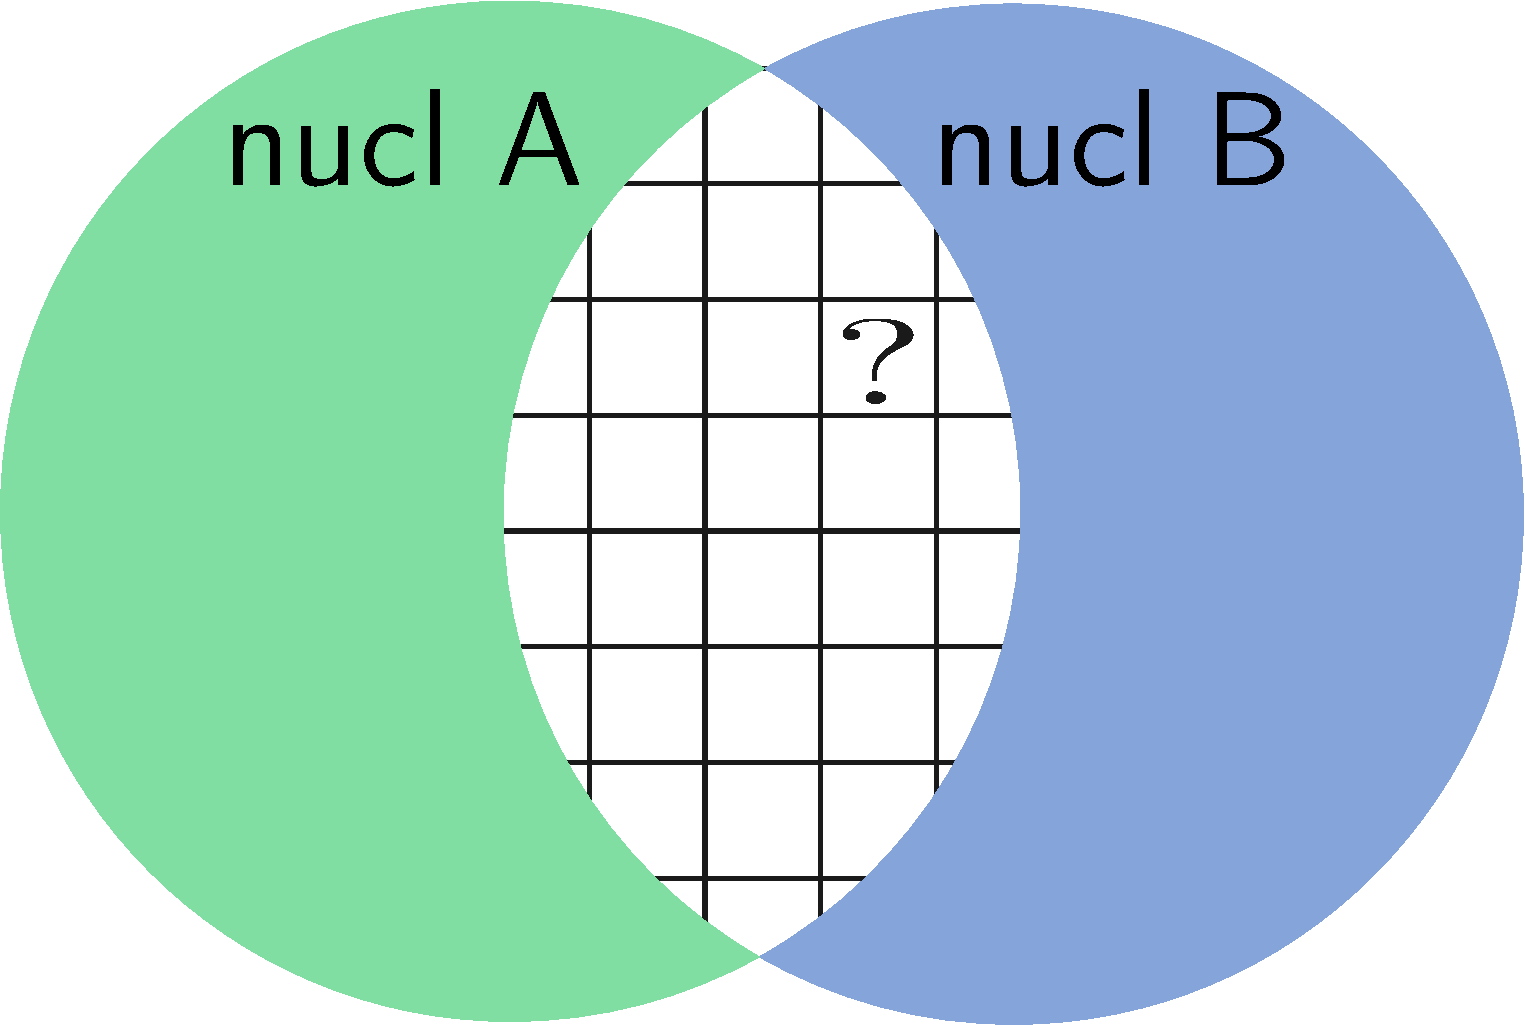
\includegraphics[width=0.28\linewidth]{motivation1}
  \end{textblock*}
 
  \begin{textblock*}{\linewidth}(0 cm, 1 cm)
  
  \only<1-3>{
  \begin{enumerate}
  \item \only<1->{Consider all combinations of m-on-n nucleon collisions, how many particles does each system produce at mid-rapidity?}
  \only<2-3>{\item Treat larger systems as amalgamation of m-on-n collisions}
  \end{enumerate}}
  \only<3->{
   \begin{block}{Fundamental assumption}
   There exists a single (possibly energy dependent) mapping from nuclear thickness to entropy density:~~ $dS/dy \vert_{y=0} \propto f(T_A,T_B)$ 
  \end{block}}
  
  \end{textblock*}

\end{frame}
%%%%%%%%%%%%%%%%%%%%%
\begin{frame}[t]{Continuous function of two variables... where to begin?}
 \vspace{0.1 in}
 \begin{itemize}
  \item For all its shortcomings, the wounded nucleon model is remarkably successful at describing soft particle production
  \item Mapping must respect basic physical constraints, e.g. symmetric and monotonic in $T_A$, $T_B$
 \end{itemize}
 \vspace{0.1 in}
 \only<2->{\centering Could start by making wild guesses ....}
 \vspace{0.1 in}
 \begin{columns}
  \begin{column}{0.33\textwidth}
    \only<2->{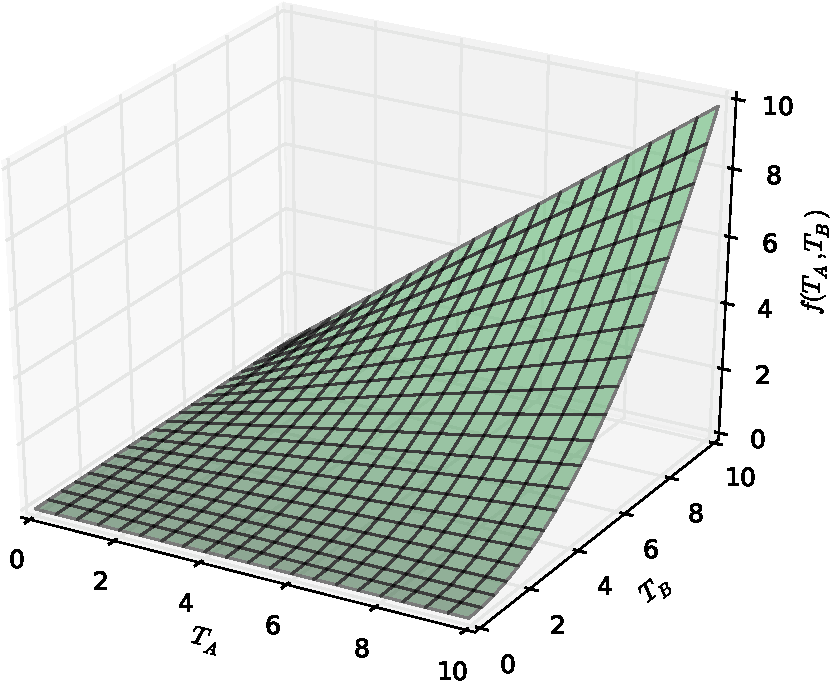
\includegraphics[width=\columnwidth]{mappings/xyy}}
  \end{column}
  \begin{column}{0.33\textwidth}
   \only<2->{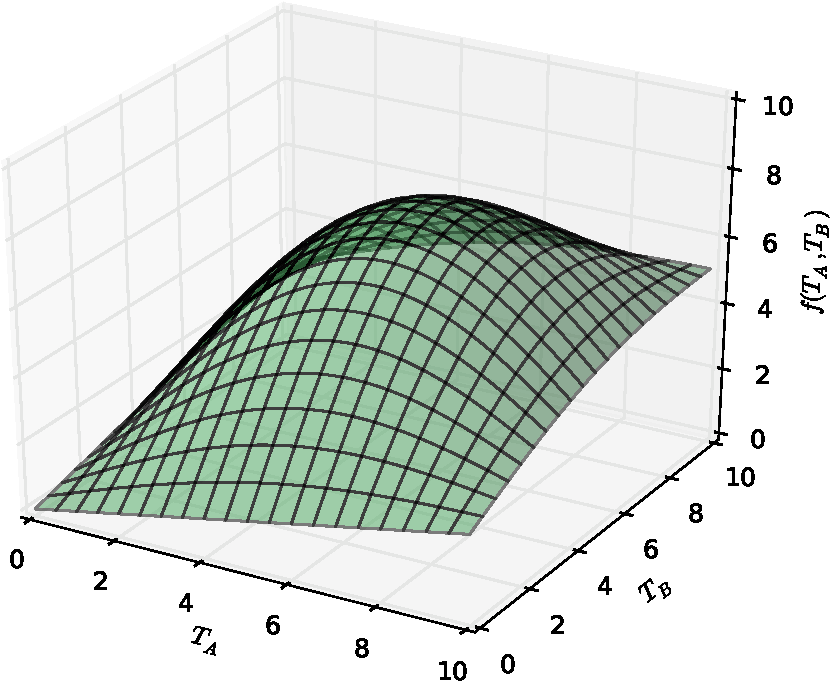
\includegraphics[width=\columnwidth]{mappings/bump}}
  \end{column}
  \begin{column}{0.33\textwidth}
   \only<2->{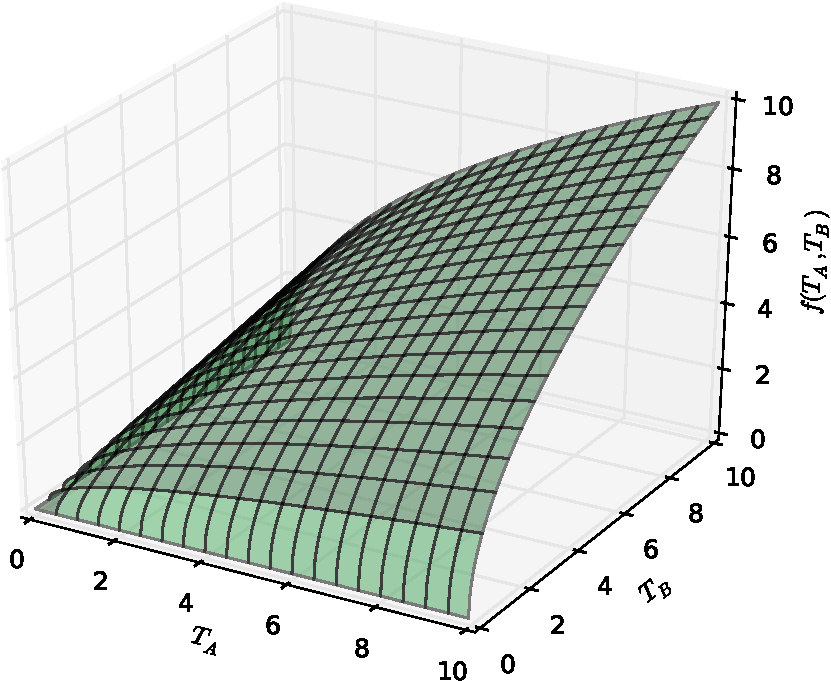
\includegraphics[width=\columnwidth]{mappings/geometric}}
  \end{column}
 \end{columns}
 
 \begin{textblock*}{\linewidth}(-4.25 cm, 0.5 cm)
  \only<3->{\fontsize{2cm}{0em} \textcolor{red}{non-symmetric}}
 \end{textblock*}
 
 \begin{textblock*}{\linewidth}(0 cm, 0.5 cm)
  \only<4->{\fontsize{2cm}{0em} \textcolor{red}{non-monotonic}}
 \end{textblock*}
 
  \begin{textblock*}{\linewidth}(4.25 cm, 0.5 cm)
  \only<5->{\fontsize{2cm}{0em} \textcolor{blue}{plausible}}
 \end{textblock*}


\end{frame}

%%%%%%%%%%%%%%%%%%%%
\begin{frame}[t]{Parameterizing entropy deposition}
 Historically started with wounded nucleon model,
 \begin{equation*}
  dS/dy \vert_{y=0} \sim \frac{T_A + T_B}{2}
 \end{equation*}
 \only<2->{
 Binary collision term later postulated to boost particle production in central A+A collisions
 \begin{equation*}
  dS/dy \vert_{y=0} \, \sim \, (1-\alpha) \frac{T_A + T_B}{2} + \alpha \, \sigma_{NN} T_A T_B
 \end{equation*}}
 \only<3->{
 In this work we replace the arithmetic mean with a generalized mean,
 \begin{equation*}
  dS/dy \vert_{y=0} \propto \left(\frac{T_A^p + T_B^p}{2}\right)^{1/p}
 \end{equation*}
 
 \begin{textblock*}{\linewidth}(0 cm, 0 cm)
  \centering
  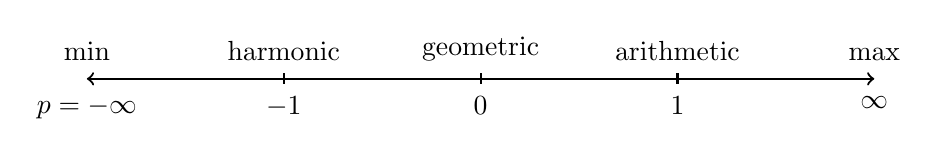
\begin{tikzpicture}
    \draw[thick,<->] (0,0) -- (10,0);
    \foreach \x in {2.5,5,7.5} \draw[thick] (\x cm,2pt) -- (\x cm,-2pt);
    \draw (0,0) node[below=3pt] {$ p=-\infty $} node[above=3pt] {min};
    \draw (2.5,0) node[below=3pt] {$ -1 $} node[above=3pt] {harmonic};
    \draw (5,0) node[below=3pt] {$ 0 $} node[above=3pt] {geometric};
    \draw (7.5,0) node[below=3pt] {$ 1 $} node[above=3pt] {arithmetic};
    \draw (10,0) node[below=3pt] {$ \infty $} node[above=3pt] {max};
  \end{tikzpicture}
\end{textblock*}
 
 }


\end{frame}


%%%%%%%%%%%%%%%%%%%%
\begin{frame}{\trento \,-- new parametric model for entropy deposition}
  \begin{textblock*}{\linewidth}(0 cm, -2.5 cm)
    \only<1->{
      \begin{enumerate}
       \small
       \only<1->{\item Sample nucleon coordinates} \vspace{0.05 in}
       \only<2->{\item Determine nucleon participants, \\ \vspace{0.05 in}
		 $P_\text{coll} = 1- \exp(-\sigma_{gg} T_{pp})$} \vspace{0.05 in}
       \only<3->{\item Define participant thickness, \\ \vspace{0.05 in}
		 $T = \sum\limits_{i=1}^{N_\text{part}} w_i T_p(x-x_i, y-y_i)$ \\ \vspace{0.05 in}
		 Sample $w_i$ from Gamma dist, \\ \vspace{0.05 in}
		 $P_k(w) = \frac{k^k}{\Gamma(k)} w^{k-1} e^{-k w}$} \vspace{0.05 in}
       \only<5->{\item Take generalized mean of $T_A, T_B$, \\ \vspace{0.05 in}
		$dS/dy \vert_{y=0} \, \propto T_R \equiv \left(\frac{T_A^p + T_B^p}{2}\right)^{1/p}$}
      \end{enumerate}}
  \end{textblock*}
  
  \begin{textblock*}{\linewidth}(0 cm, 4 cm)
    \centering \only<10->{``Thickness Reduced Event-by-event Nuclear Topology''}
  \end{textblock*}

   \begin{textblock*}{0.5\linewidth}(5.65 cm, -2.5 cm)
    \only<1>{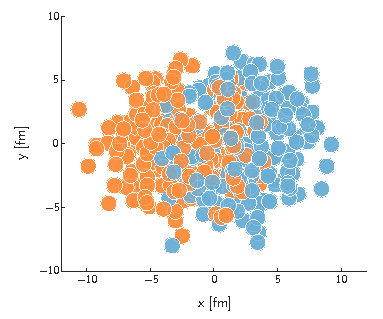
\includegraphics[width=\linewidth]{process0}}
    \only<2>{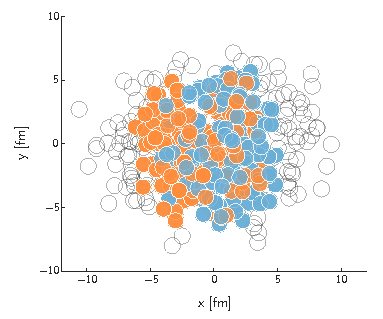
\includegraphics[width=\linewidth]{process1}}
    \only<3>{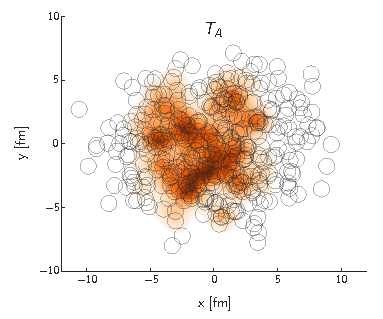
\includegraphics[width=\linewidth]{process2}}
    \only<4>{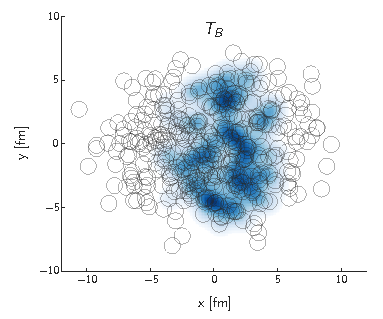
\includegraphics[width=\linewidth]{process3}}
    \only<5>{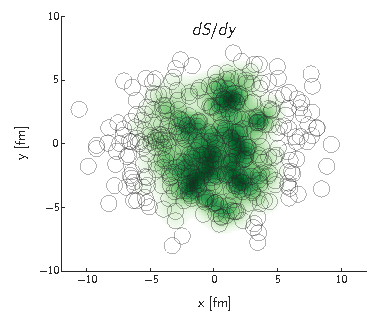
\includegraphics[width=\linewidth]{thickness}}
    \only<6>{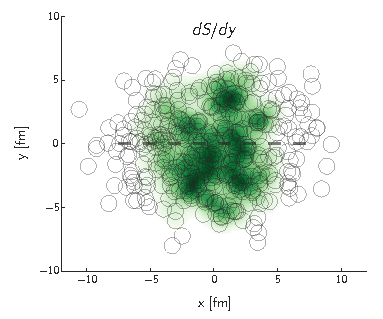
\includegraphics[width=\linewidth]{thickness2}}
    \only<7>{\vspace{0.06 in} 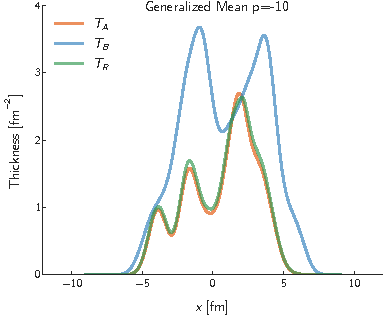
\includegraphics[width=\linewidth]{xs_-10}}
    \only<8>{\vspace{0.06 in} 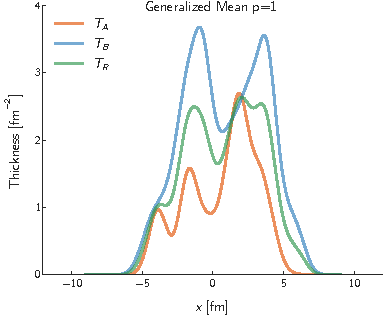
\includegraphics[width=\linewidth]{xs_1}}
    \only<9>{\vspace{0.06 in} 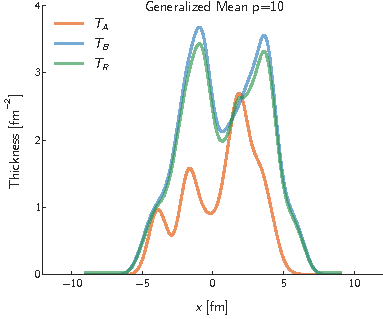
\includegraphics[width=\linewidth]{xs_10}}
    \only<10->{\vspace{0.06 in} 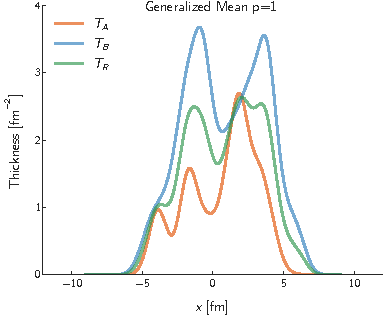
\includegraphics[width=\linewidth]{xs_1}}
   \end{textblock*}
\end{frame}

%%%%%%%%%%%%%%%%%%%

\begin{frame}{Demonstrating the flexibility of the ansatz}
 \begin{itemize}
  \item For $p=1$ model reduces to a wounded nucleon model (exact)
  \item for $p=-0.65$ model replicates the KLN mapping to $\mathcal{O}(1\%)$
 \end{itemize}
 \vspace{-0.2 in}
 \begin{eqnarray*}
  \cr \frac{dN_g}{d^2 r_\perp dy} &\sim& Q^2_{s,min} \left(2 + \log \left(\frac{Q^2_{s,max}}{Q^2_{s,min}} \right) \right), \quad Q_s^2 \sim T
 \end{eqnarray*}
 \vspace{-0.1 in} \centering \footnotesize Drescher, Nara Phys. Rev. C {\bf 75}, 034905 (2007)
 \vspace{0.3 in}
 \begin{columns}
  \begin{column}{0.4\textwidth}
    \centering \footnotesize KLN mapping \\
    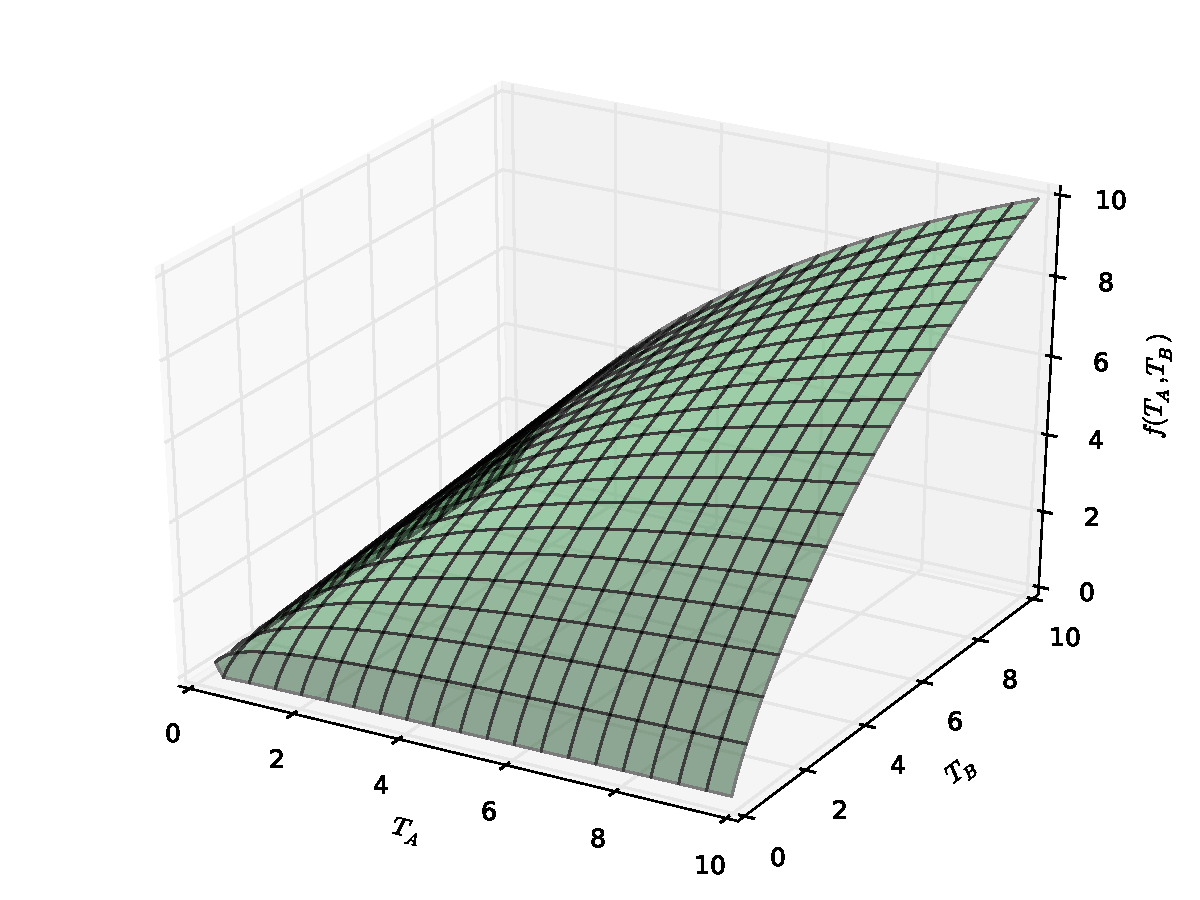
\includegraphics[width=\linewidth]{KLN}
  \end{column}
  \begin{column}{0.4\textwidth}
   \centering \footnotesize Generalized mean p=-0.65
   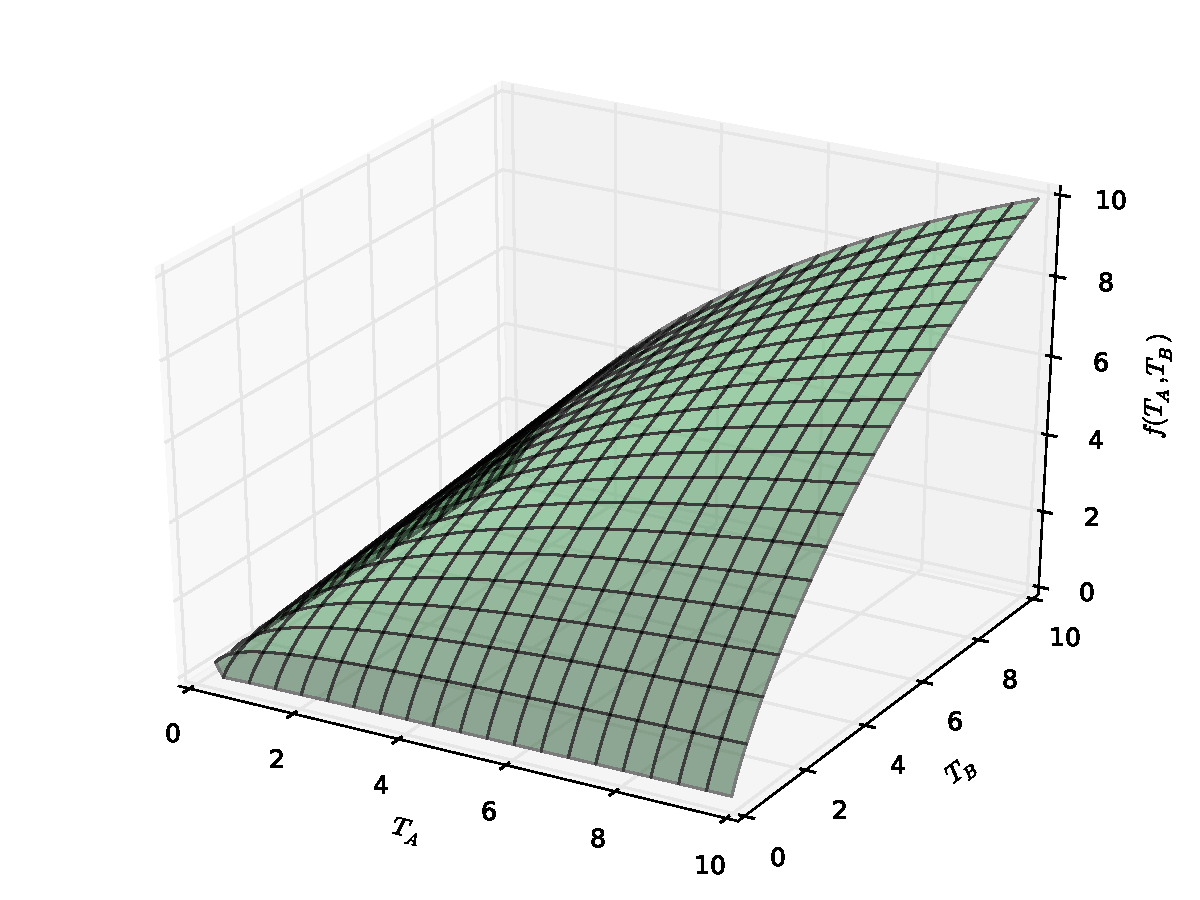
\includegraphics[width=\linewidth]{KLN}
  \end{column}

 \end{columns}

\end{frame}

\begin{frame}[t]{Demonstrating the flexibility of the ansatz}
  \begin{columns}
   \begin{column}{0.55\textwidth}
    \vspace{-1 in}
    \begin{itemize}
     \item $p \approx 0$ mimics the IP-Glasma model
     \vspace{0.05 in}
     \item Similar harmonics and multiplicities \\
	  right: eccentricity vs impact param. \\
     \vspace{0.05 in}
     \item More on this later in the talk ...
    \end{itemize}
   \end{column}
   \begin{column}{0.45\textwidth}
    \centering 
    \vspace{0.05 in}
    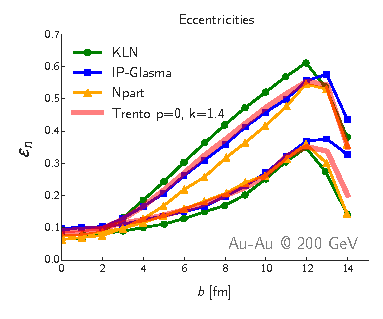
\includegraphics[width=\columnwidth]{trento-v-glasma} \\
    {\scriptsize Schenke, Tribedy, Venugopalan \\ Phys. Rev. Lett.  {\bf 108}, 252301 (2012) }
   \end{column}

  \end{columns}
  
  \vspace{0.2 in}
  \emph{Opportunity: Constrain the generalized mean parameter p via systematic model-to-data comparison to simultaneously extract the QGP viscosity and 
    initial conditions}


  
\end{frame}



%%%%%%%%%%%%%%%%%%%

\begin{frame}[t, label=nch]{Testing parameterization against measured multiplicities}
 
 \centering \vspace{0.05 in} \hspace{-0.2 in}
 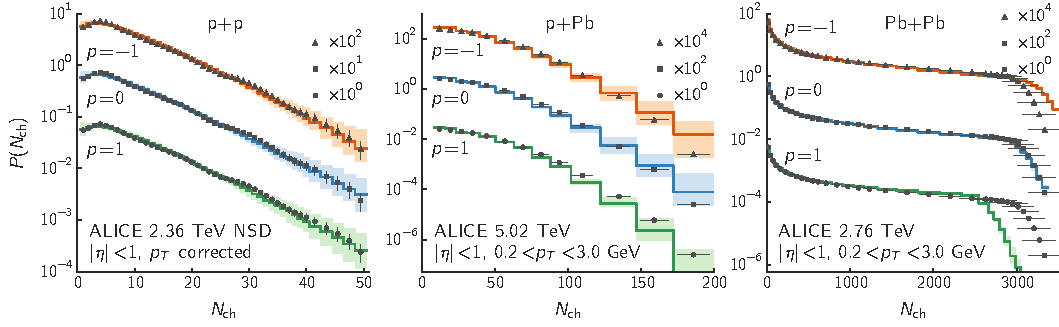
\includegraphics[scale=0.675]{nch}
 
  \begin{textblock*}{\linewidth}(0.0 cm, 0.5 cm)
    \only<1-4>{\centering \trento\, model plotted against LHC multiplicity distributions}
    
    \only<2-4>{
    \begin{itemize}
      \only<2-4>{\item Lines indicate different values of the generalized mean (annotated)}
      \vspace{0.05 in}
      \only<3-4>{\item Bands indicate $\pm 30\%$ variation in optimal fluctuation parameter}
      \vspace{0.05 in}
      \only<4>{\item Norm is varied to account for differences in energy and kinematic cuts}
    \end{itemize}}
    
  \end{textblock*}
 
  \only<5>{
  \begin{textblock*}{\linewidth}(0.65 cm, -4.17 cm)
    \flushleft
    \begin{tikzpicture}
      \draw[purple,thick] (0,0) -- (7.28,0) -- (7.28,3.1) -- (0,3.1) -- (0,0);
    \end{tikzpicture}
  \end{textblock*}}
  
  \only<6>{
  \begin{textblock*}{\linewidth}(8.53 cm, -4.17 cm)
    \flushleft
    
\begin{tikzpicture}
      \draw[purple,thick] (0,0) -- (3.36,0) -- (3.36,3.1) -- (0,3.1) -- (0,0);
    \end{tikzpicture}
  \end{textblock*}}
    
  \begin{textblock*}{\linewidth}(0.0 cm, 0.5 cm)
    \vspace{-0.082 in}
    \only<5->{ 
    \begin{itemize}
      \only<5->{\item All means fit p+p, p+Pb with suitably chosen norm and fluctuations}
      \only<6->{\item Only geometric mean describes shape of Pb+Pb data} 
      \only<7->{\item Normalizations provide further constraints on allowable parameters:}
    \end{itemize}}
    \vspace{-0.18 in}
    \only<7->{
      \begin{table}[t]
          \small
	  \begin{tabular}{rcccc}
	    $p\;$  & $k$ & p+p norm & p+Pb norm & Pb+Pb norm \\
	    \noalign{\smallskip}\hline\noalign{\smallskip}
	    $+1$   & 0.8 & 9.7      & \only<7>{\textcolor{black}{7.0}}\only<8>{\textcolor{red}{7.0}} & \only<7>{\textcolor{black}{13.}}\only<8>{\textcolor{red}{13.}}        \\
	    $ 0$   & 1.4 & 19.      & 17.       & 16.        \\
	    $-1$   & 2.2 & 24.      & 26.       & 18.        \\
	  \end{tabular}
      \end{table}
    }

  \end{textblock*}
 
\end{frame}


%%%%%%%%%%%%%%%%%%%
\begin{frame}[t]{Testing parameterization against flow constraints}
 \centering \vspace{0.2 in} \hspace{-0.2 in}
 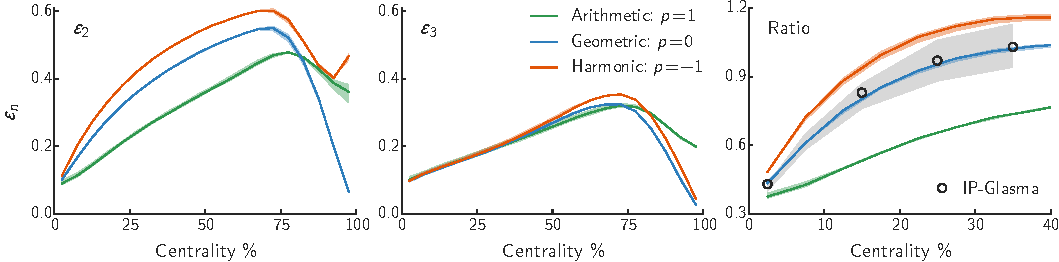
\includegraphics[scale=0.675]{eccentricity}
 
  \begin{textblock*}{\linewidth}(4.01 cm, -3.25 cm)
   \tiny Gray band: PRC {\bf 89} 014902 (2014) 
  \end{textblock*}

 
  \begin{textblock*}{\linewidth}(0.0 cm, 0.5 cm)
    
    \only<1-4>{\trento \, Pb+Pb eccentricity harmonics: 
    $\varepsilon_n e^{i n \phi} = -\frac{\int dx\, dy\, r^n e^{i n \phi} s(x,\,y)}{\int dx\, dy\, r^n s(x,\, y)} $}
    
    \only<2-4>{
      \begin{itemize}
       \item \only<2->{Generalized mean parameter strongly affects fireball ellipticity,}
       \only<3->{but only weakly affects triangularity}
       \only<4->{\item Varying fluctuation parameter by $\pm 30 \%$ has negligible effect on \\
		       eccentricity harmonics, i.e. p+p fluctuations are sub-leading effect.}
      \end{itemize}}

    \only<5->{Ratio of $\varepsilon_2/\varepsilon_3$ strong discriminator for initial condition models. \\
	      Easy to fit $v_2$ by varying $\eta/s$... hard to fit $v_2$ and $v_3$ simultaneously.}
	      
    \only<6->{
      \begin{itemize}
       \item  Gray band from Retinskaya, Luzum, Ollitrault, allowed region for eccentricity ratio 
	      {\small $\sqrt{\langle \varepsilon_2^2 \rangle}/\sqrt{\langle \varepsilon_3^2 \rangle}^{0.6}$} determined using measured flows and linear response $v_n \propto \varepsilon_n$.  
       \item Eccentricity ratio prefers geometric mean and mimics IP-Glasma \\ 
	     Both multiplicities and flows in agreement, prefer $p \sim 0$ at LHC
      \end{itemize}}
    
  \end{textblock*}
  
  \only<2>{
  \begin{textblock*}{\linewidth}(0.38 cm, -3.4 cm)
    \flushleft
    
\begin{tikzpicture}
      \draw[purple,thick] (0,0) -- (3.45,0) -- (3.45,2.4) -- (0,2.4) -- (0,0);
    \end{tikzpicture}
  \end{textblock*}}
  
  \only<3>{
  \begin{textblock*}{\linewidth}(4.36 cm, -3.4 cm)
    \flushleft
    
\begin{tikzpicture}
      \draw[purple,thick] (0,0) -- (3.45,0) -- (3.45,2.4) -- (0,2.4) -- (0,0);
    \end{tikzpicture}
  \end{textblock*}}
  
  \only<5->{
  \begin{textblock*}{\linewidth}(8.326 cm, -3.4 cm)
    \flushleft
    
\begin{tikzpicture}
      \draw[purple,thick] (0,0) -- (3.45,0) -- (3.45,2.4) -- (0,2.4) -- (0,0);
    \end{tikzpicture}
  \end{textblock*}}
 
\end{frame}

%%%%%%%%%%%%%%%%%%

\begin{frame}[t]{Event-by-event flow distributions}
 Top: IP-Glasma $\varepsilon_2/\langle \varepsilon_2 \rangle$, and IP-Glasma+Music $v_2/\langle v_2 \rangle$ ({\footnotesize Bjorn's QM14 talk}) \\
 \vspace{0.05 in}
 Bottom: \trento\, $\varepsilon_2/\langle \varepsilon_2 \rangle$ for different values of the generalized mean \\
 \vspace{0.1 in}
 \begin{columns}
  \begin{column}{0.33\textwidth}
    \centering 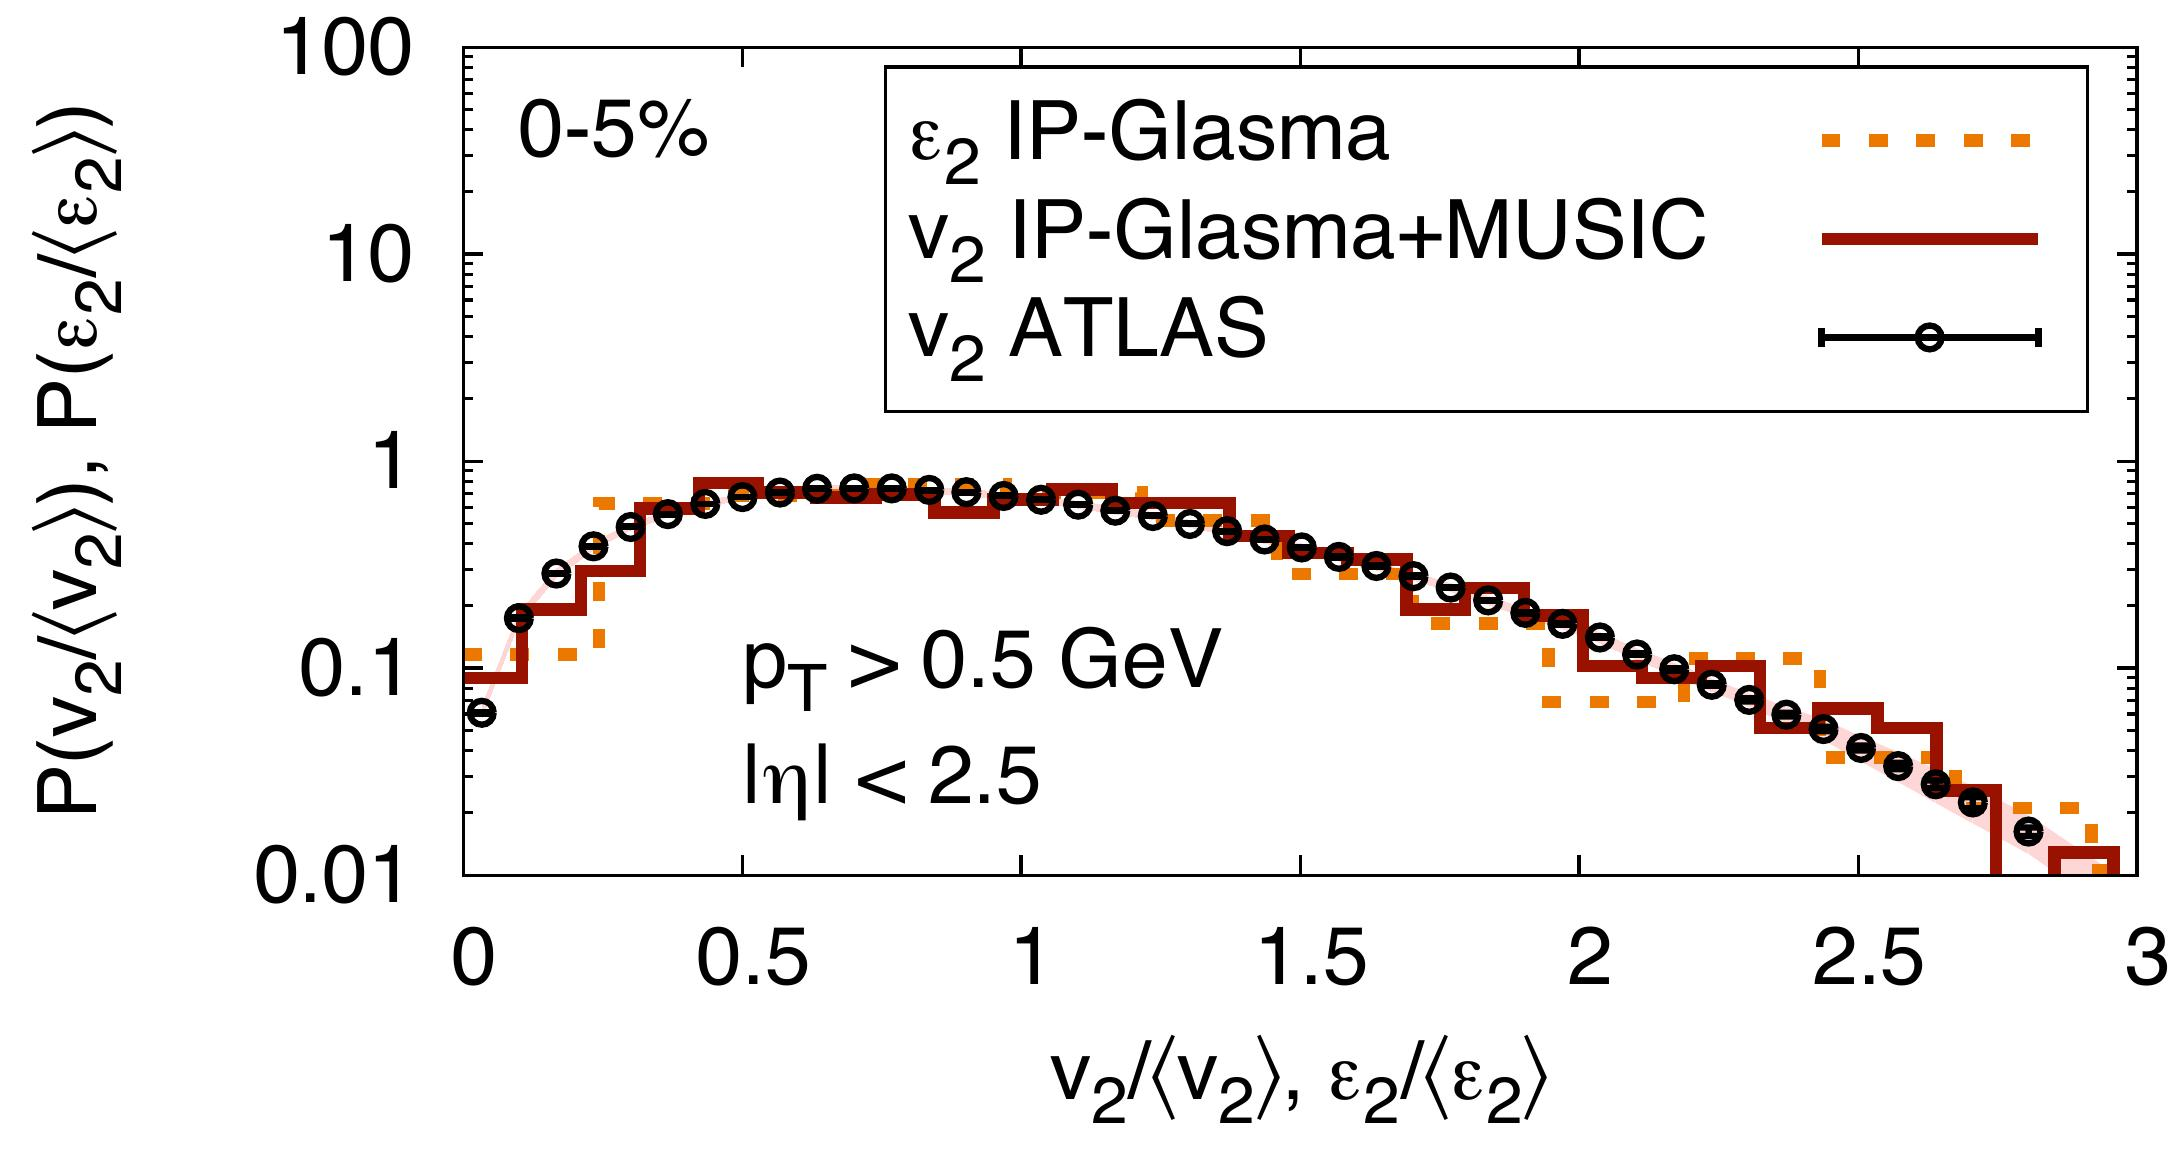
\includegraphics[width=\columnwidth]{ebe-flow/bjorn_01}
  \end{column}
  \begin{column}{0.33\textwidth}
    \centering 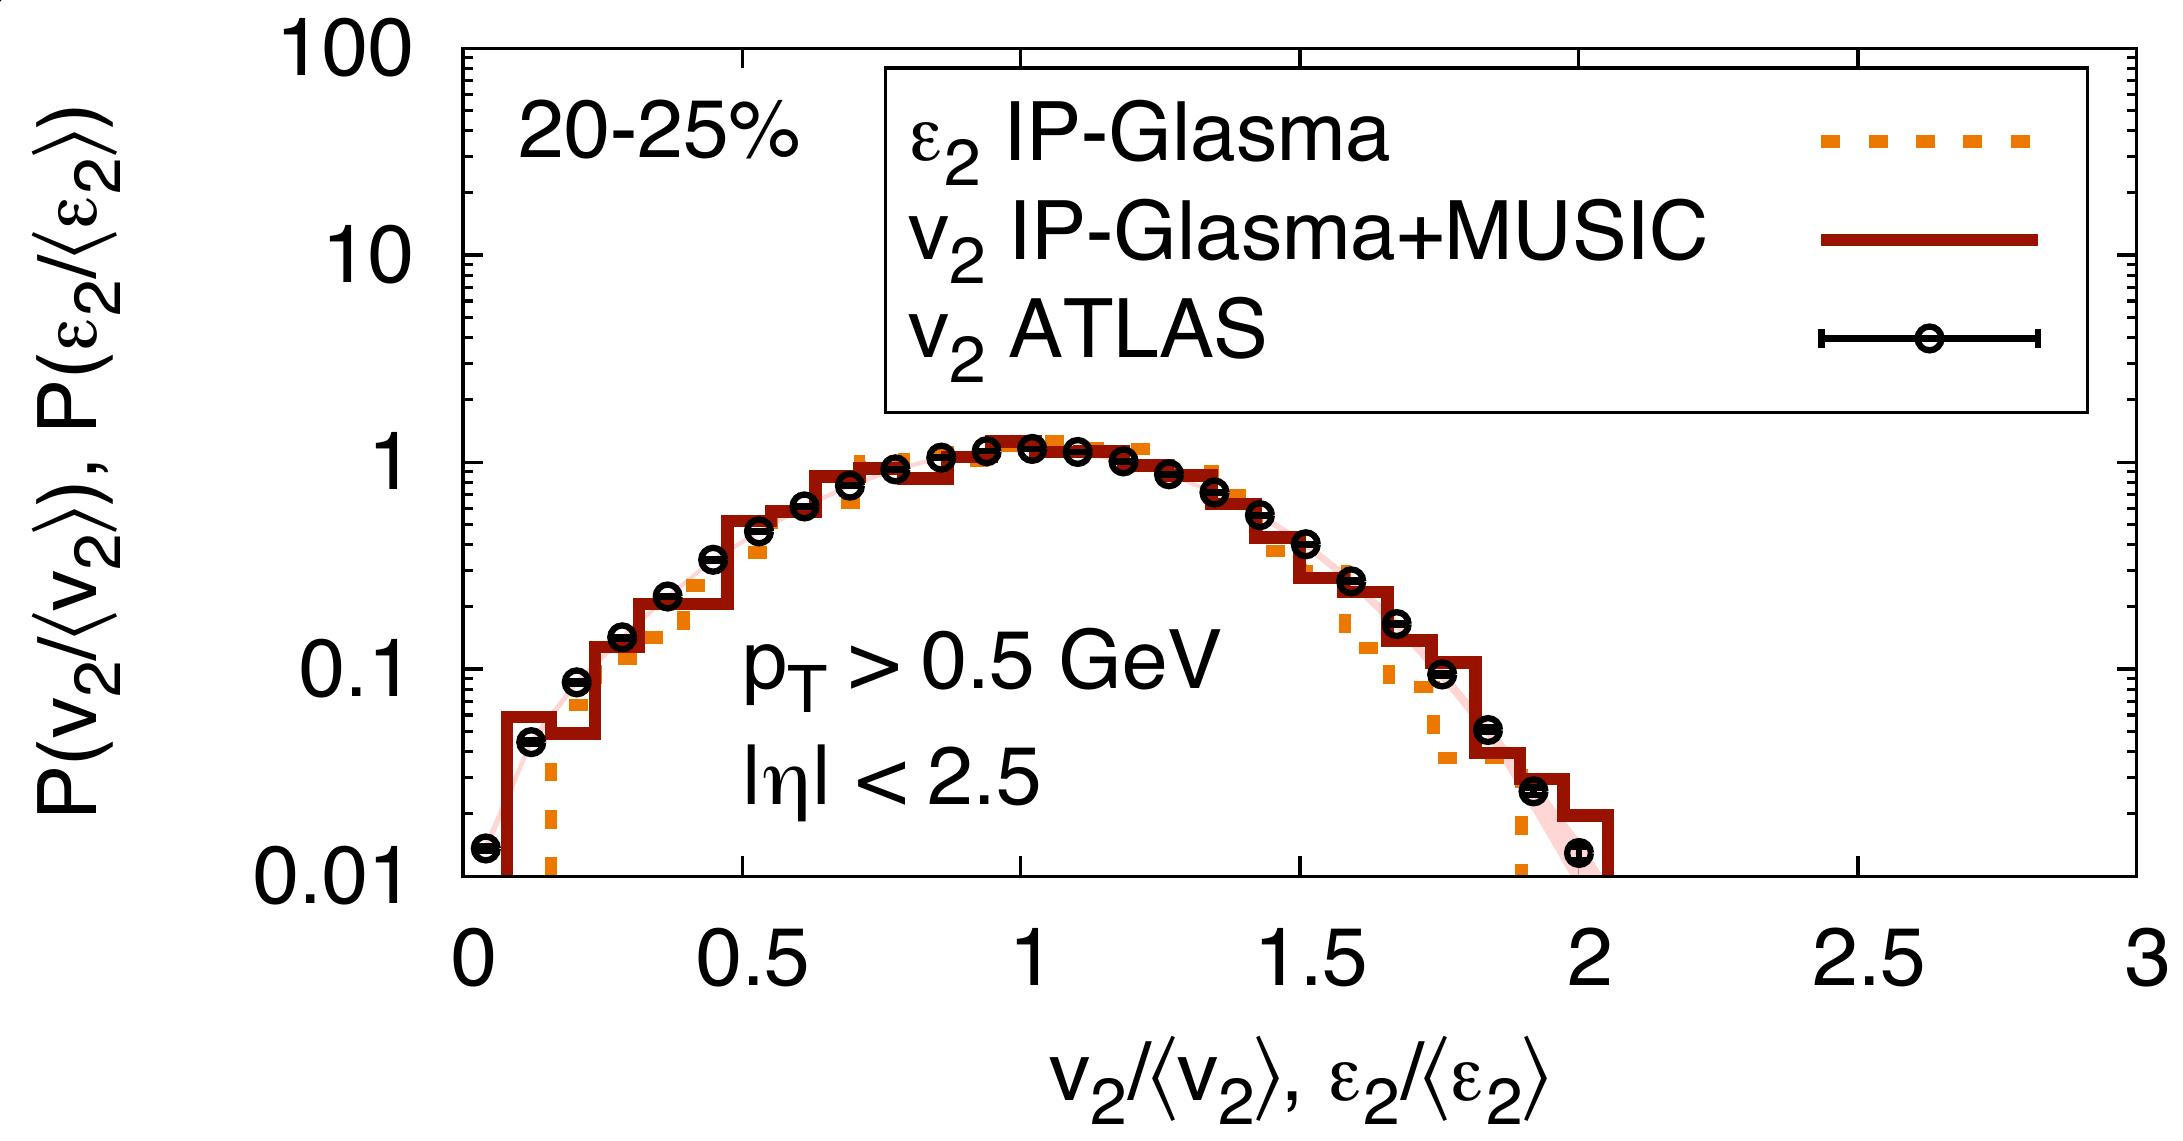
\includegraphics[width=\columnwidth]{ebe-flow/bjorn_02}
  \end{column}
  \begin{column}{0.33\textwidth}
    \centering 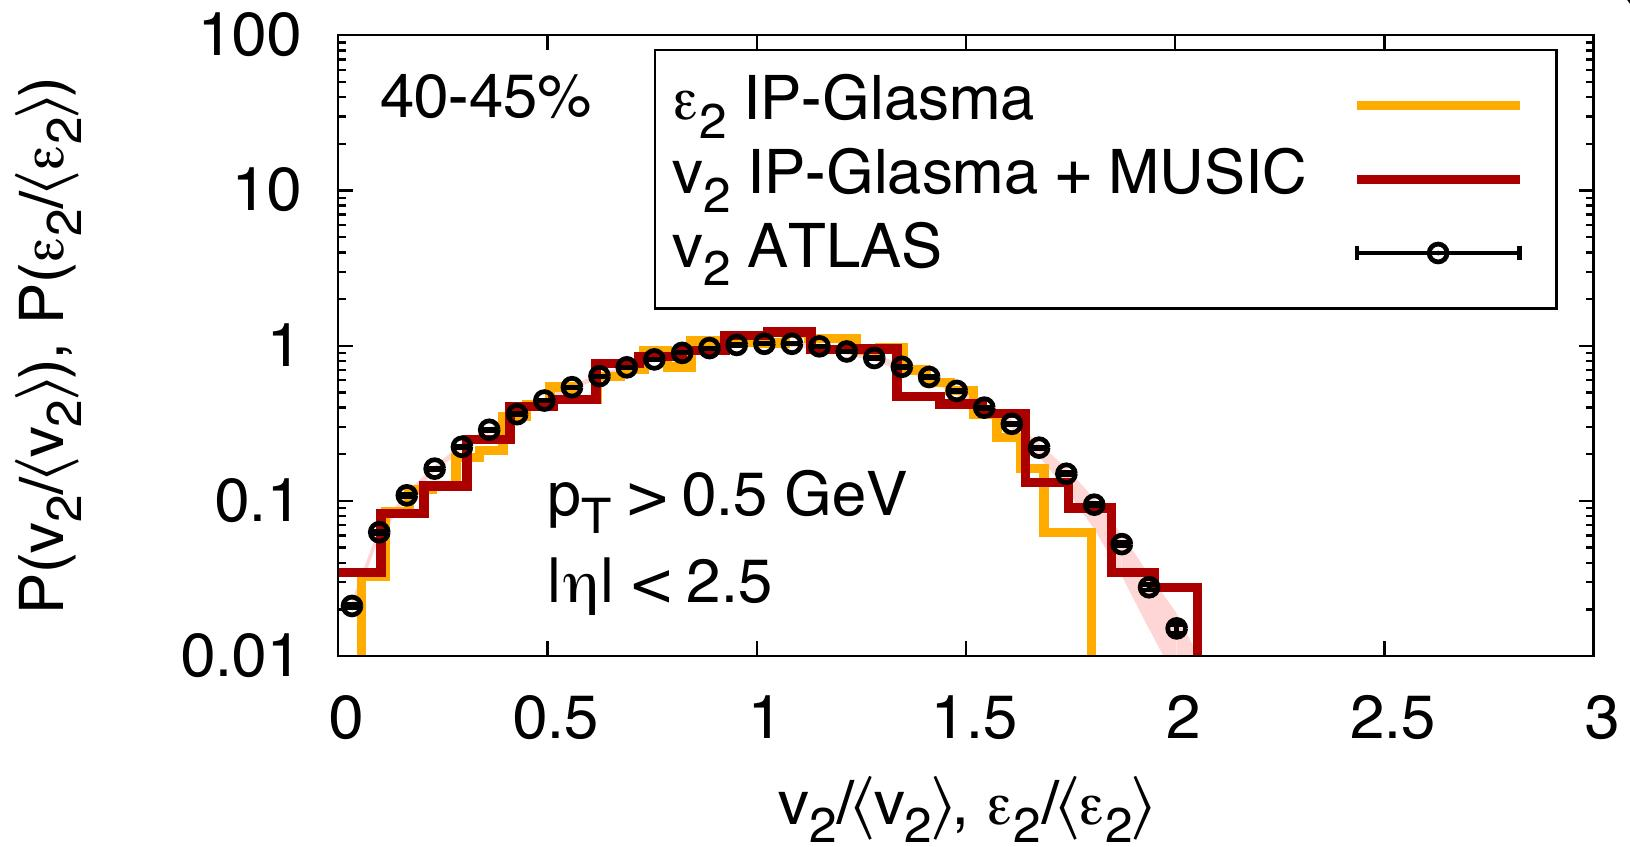
\includegraphics[width=\columnwidth]{ebe-flow/bjorn_03}
  \end{column}
 \end{columns}
 \vspace{0.1 in}
  \begin{columns}
  \begin{column}{0.33\textwidth}
    \centering 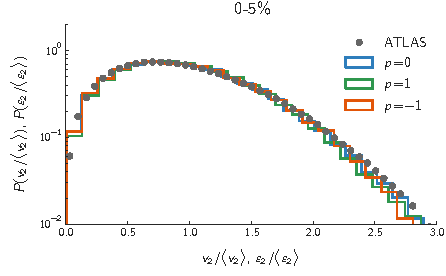
\includegraphics[width=\columnwidth]{ebe-flow/v2_02}
  \end{column}
  \begin{column}{0.33\textwidth}
    \centering 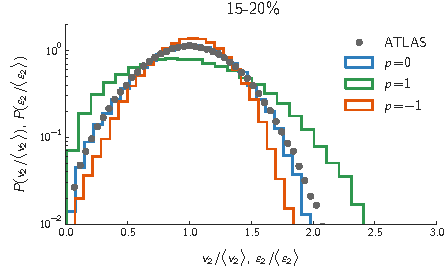
\includegraphics[width=\columnwidth]{ebe-flow/v2_09}
  \end{column}
  \begin{column}{0.33\textwidth}
    \centering 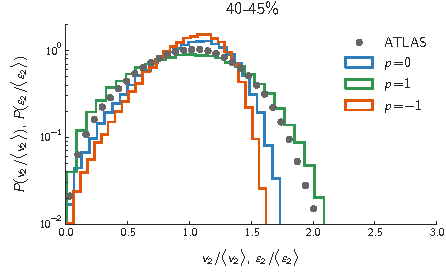
\includegraphics[width=\columnwidth]{ebe-flow/v2_14}
  \end{column}
 \end{columns}
 \vspace{0.1 in}
 \only<2->{
 Generalized mean parameter strongly affects eccentricity distribution shape. Preliminary results (no hydro) consistent 
 with $p \approx 0$. Consistent with harmonic ratio and multiplicity constraints shown previously.}
\end{frame}

%%%%%%%%%%%%%%%%%%%%%
\begin{frame}[plain]
 \centering \LARGE Implications for small collision systems
\end{frame}

%%%%%%%%%%%%%%%%%%%
\newcommand{\ppoverlap}[1]{#1}

\begin{frame}[label=ppoverlap]{Mapping effect on p+p entropy deposition}

  \begin{textblock*}{\linewidth}(-3.5 cm, -2.75 cm)
    \centering 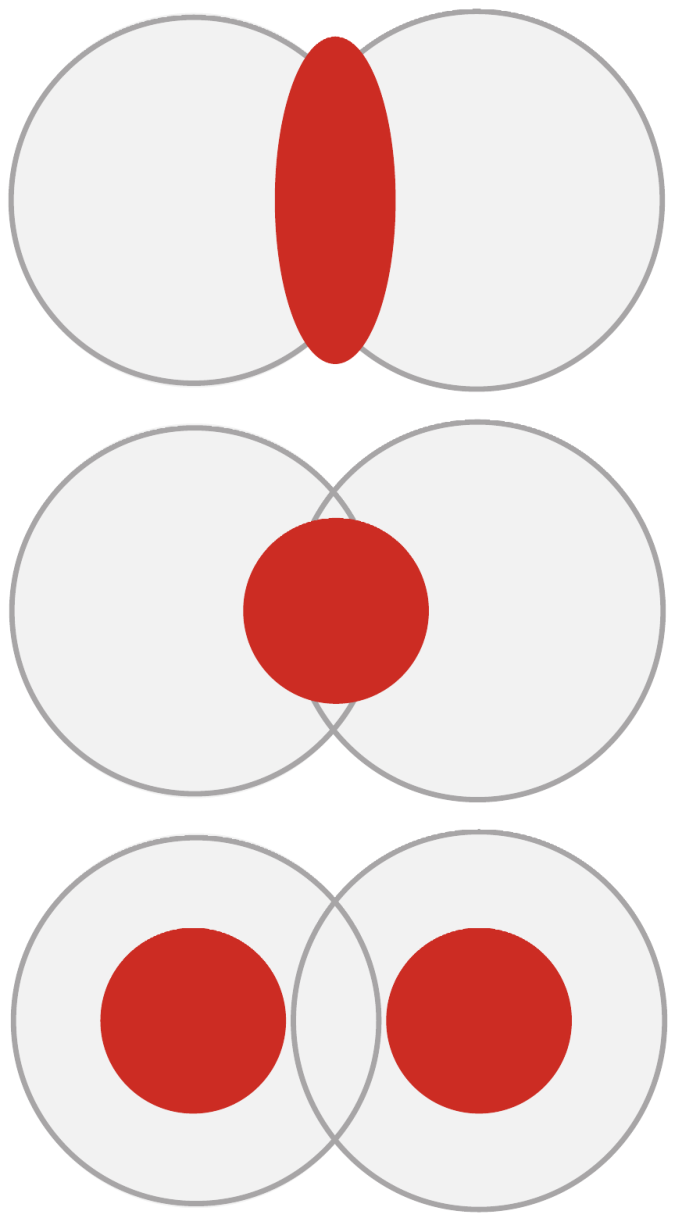
\includegraphics[scale=0.25]{bjorn-shapes} \\
    \vspace{0.1 in}
    \tiny Bzdak, Schenke, Tribedy, Venugopalan, \\
    Phys.\ Rev.\ C {\bf 87}, no. 6, 064906 (2013)
  \end{textblock*}
  
  \begin{textblock*}{\linewidth}(2.25 cm, -2.9 cm)
    \centering Generalized Mean p+p collision 
  \end{textblock*}

 
  \begin{textblock*}{\linewidth}(4.5 cm, -2.5 cm)
    \only<1>{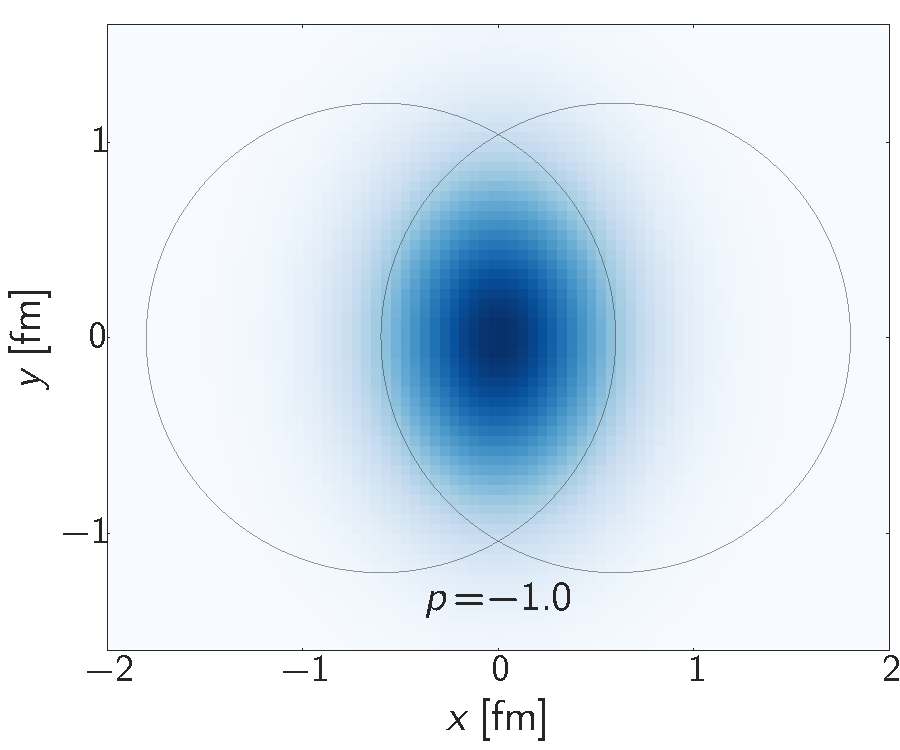
\includegraphics[scale=0.45]{pg_0001}}
    \only<2>{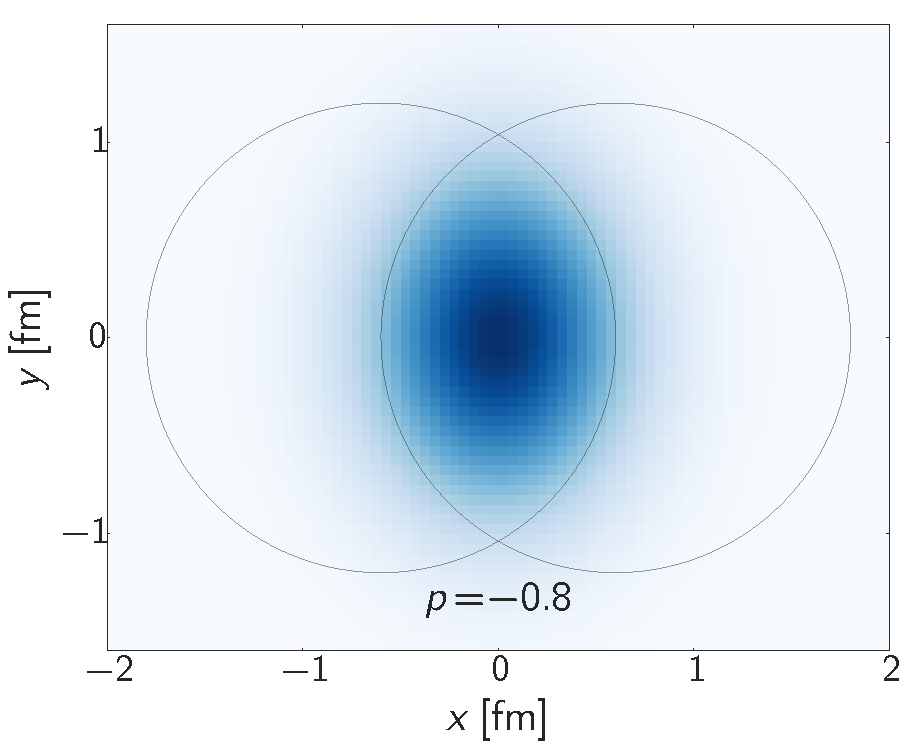
\includegraphics[scale=0.45]{pg_0002}}
    \only<3>{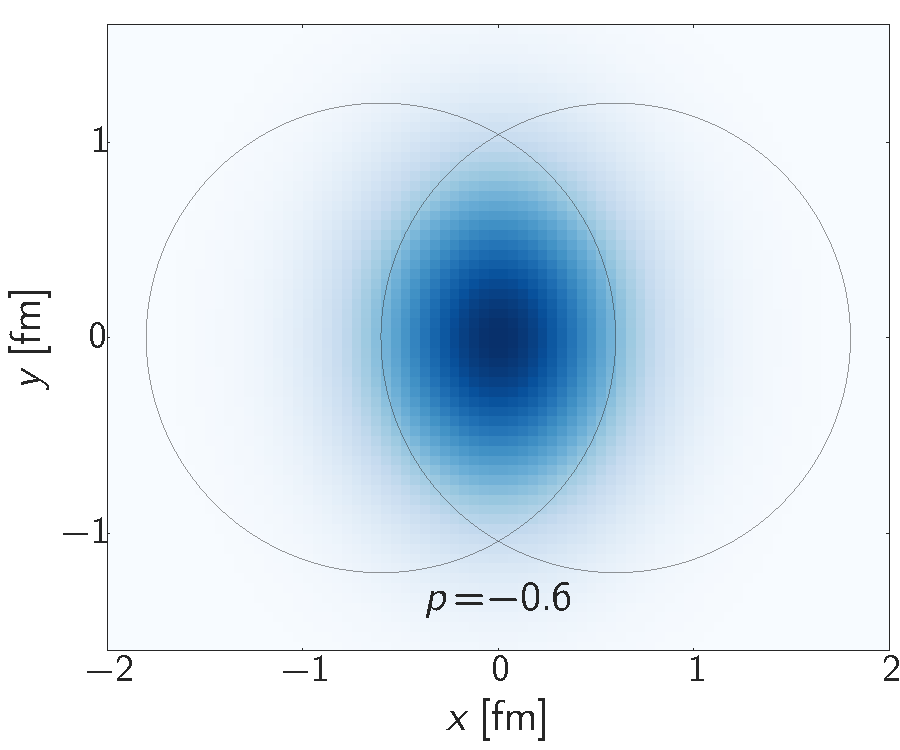
\includegraphics[scale=0.45]{pg_0003}}
    \only<4>{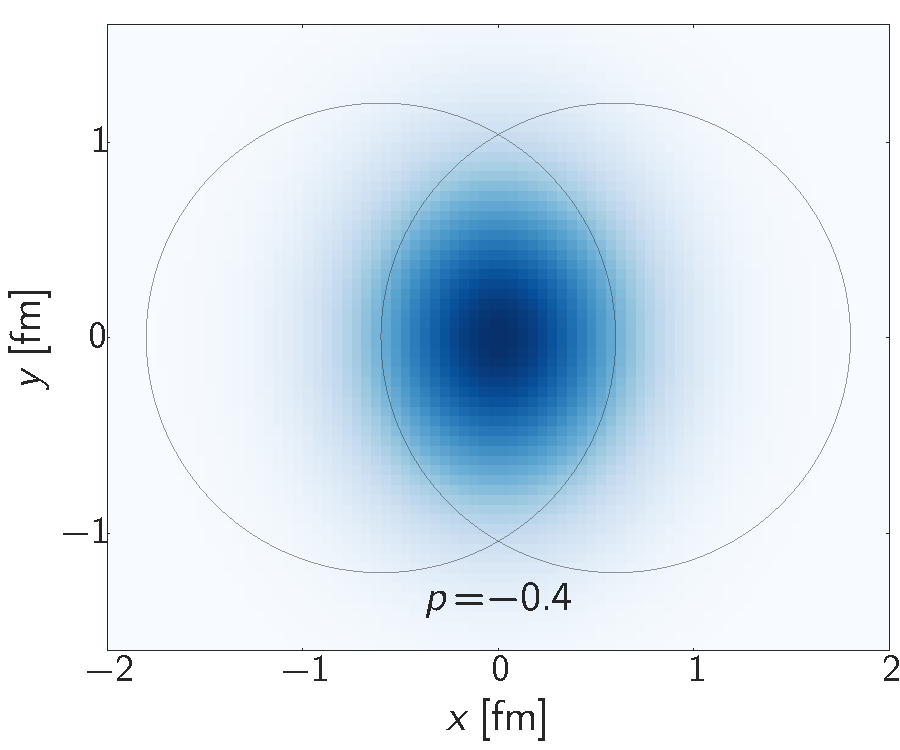
\includegraphics[scale=0.45]{pg_0004}}
    \only<5>{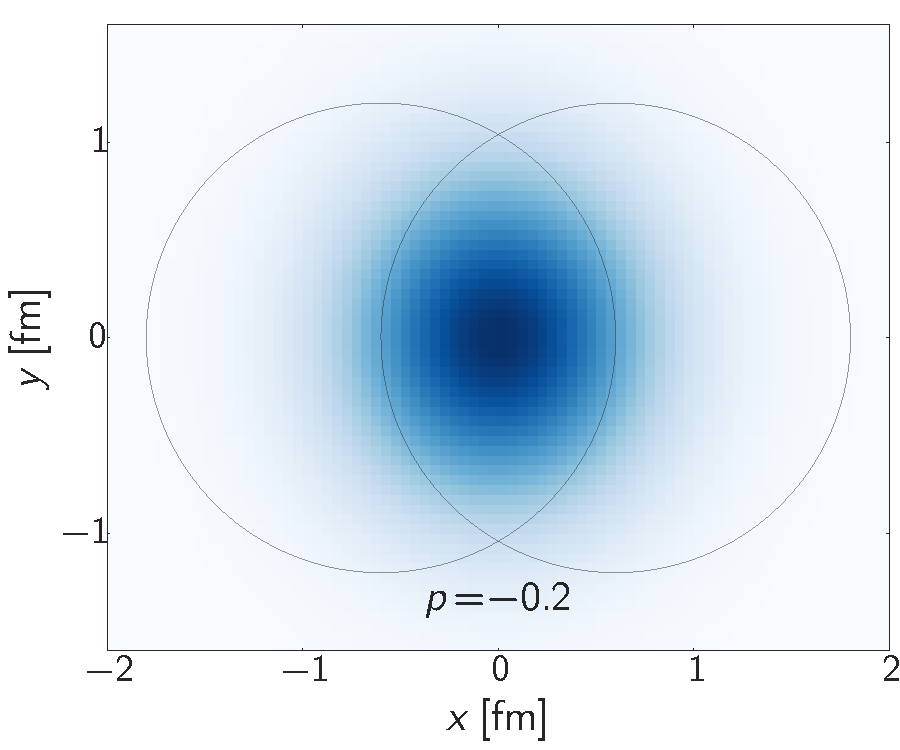
\includegraphics[scale=0.45]{pg_0005}}
    \only<6>{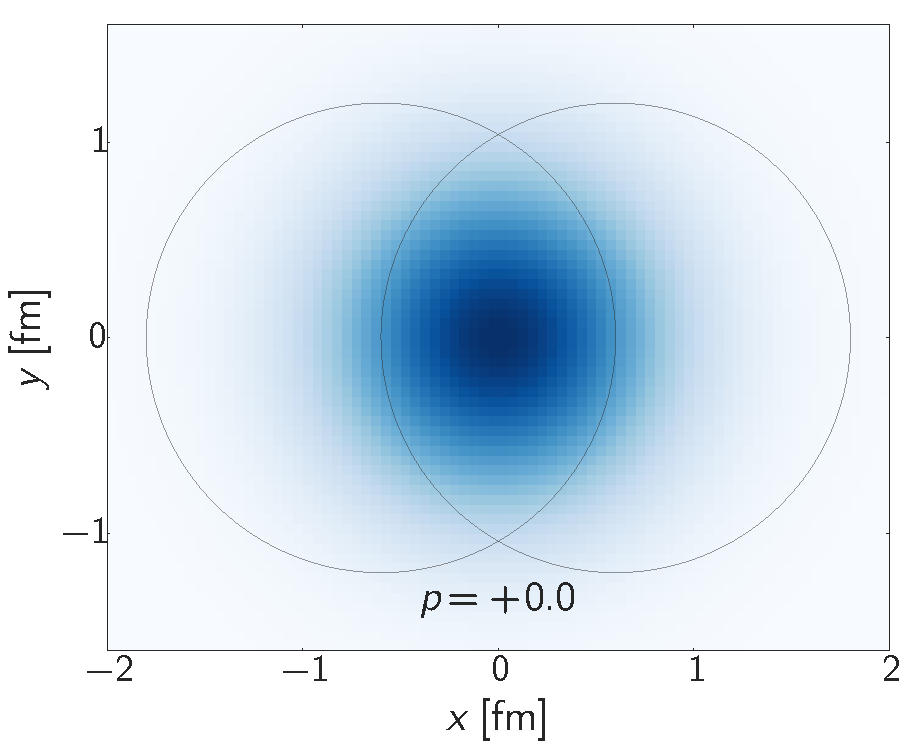
\includegraphics[scale=0.45]{pg_0006}}
    \only<7>{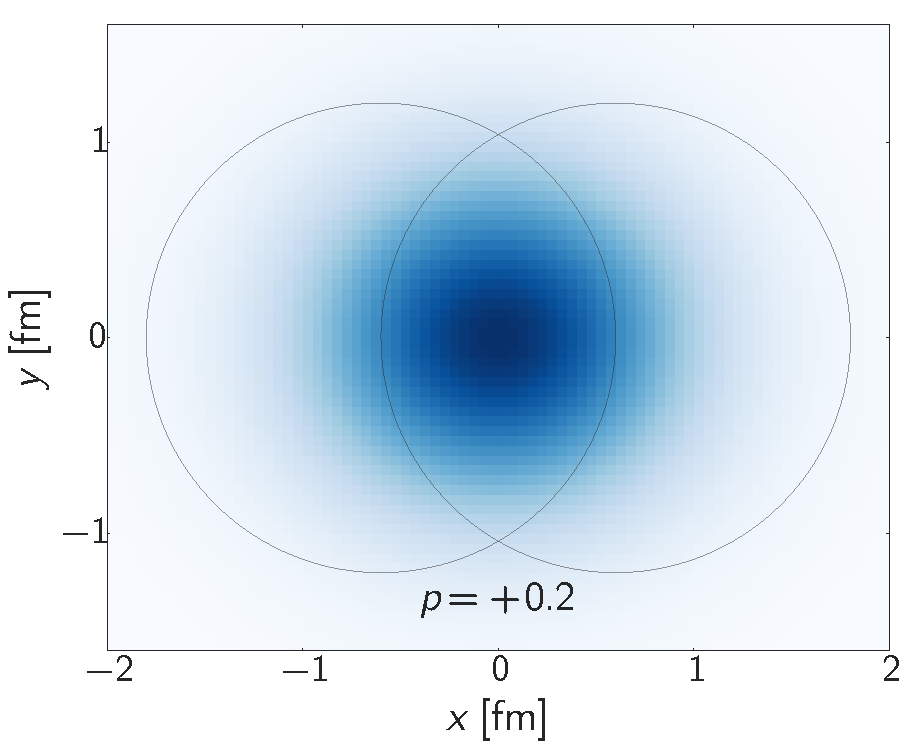
\includegraphics[scale=0.45]{pg_0007}}
    \only<8>{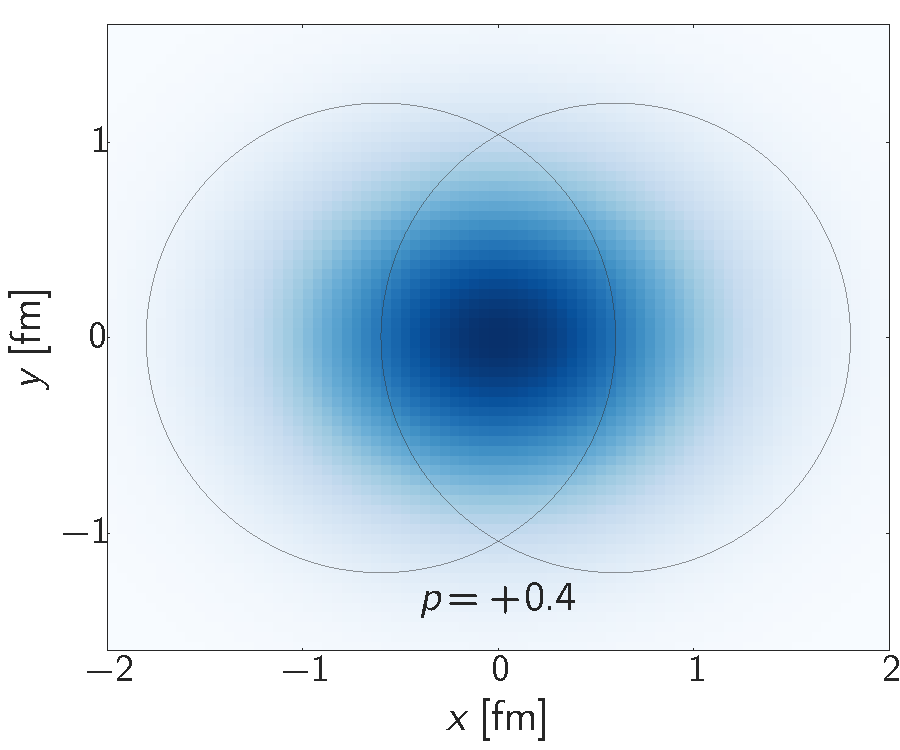
\includegraphics[scale=0.45]{pg_0008}}
    \only<9>{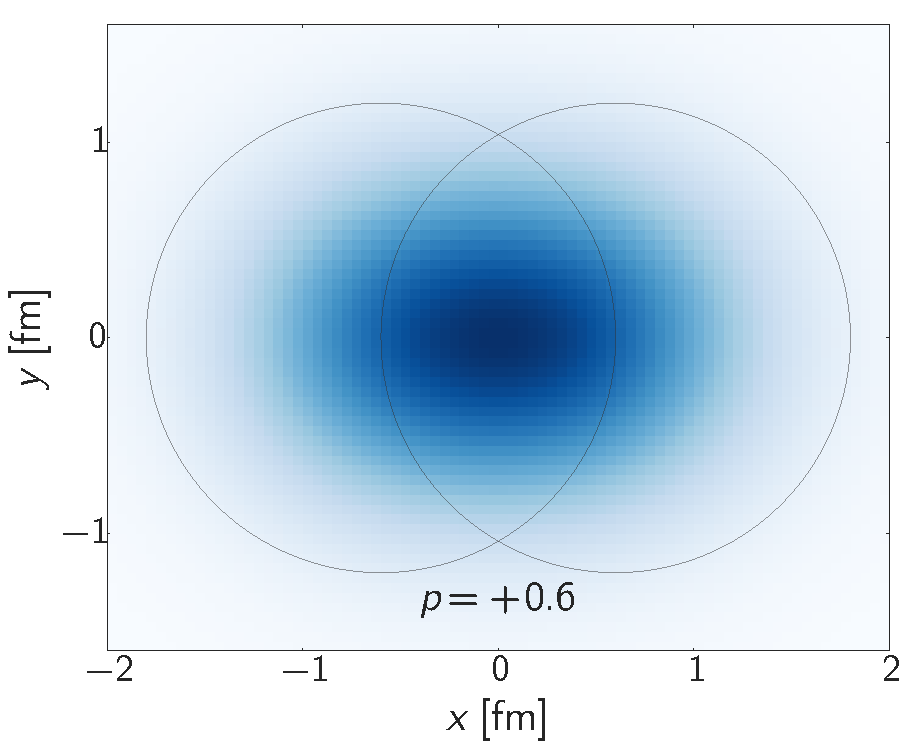
\includegraphics[scale=0.45]{pg_0009}}
    \only<10>{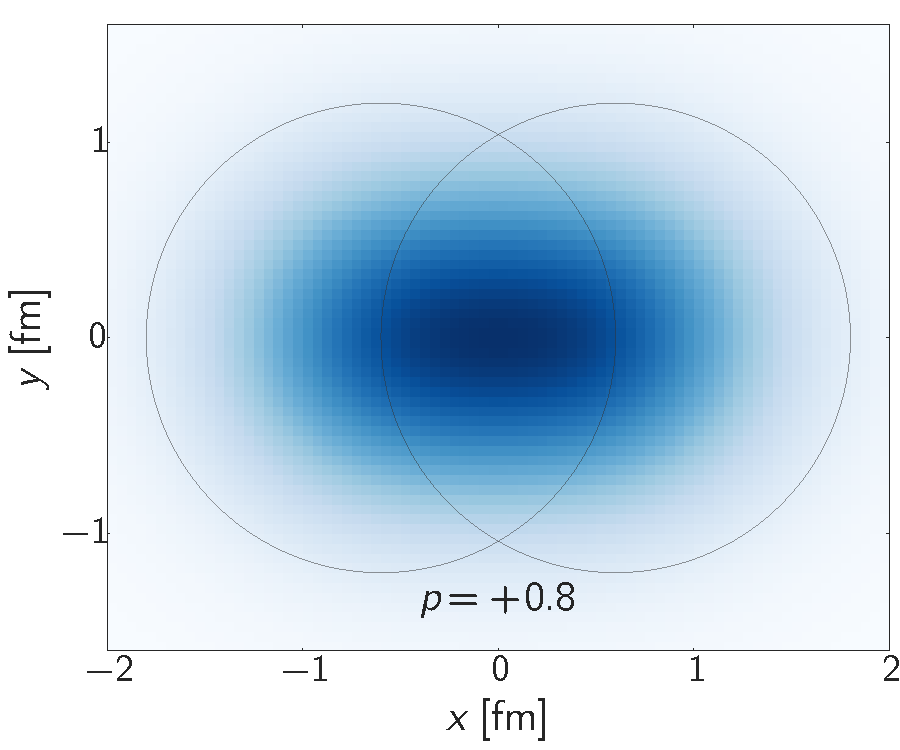
\includegraphics[scale=0.45]{pg_0010}}
    \only<11>{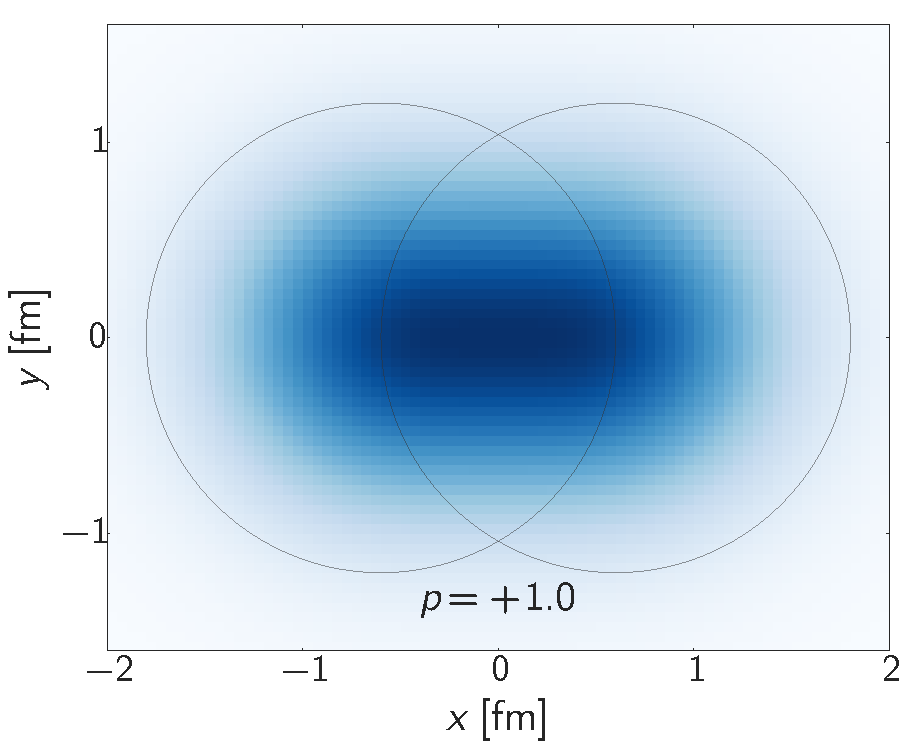
\includegraphics[scale=0.45]{pg_0011}}
  \end{textblock*}

  \begin{textblock*}{\linewidth}(0.0 cm, 4 cm)
    \centering Generalized mean interpolates between distinct deposition schemes
  \end{textblock*}
 
\end{frame}


%%%%%%%%%%%%%%%%%%%
\newcommand{\meanmarker}[1]{#1}
\newcommand{\pPb}[1]{#1}
\newcommand{\dAu}[1]{#1}

\begin{frame}[label=pvariation]

\begin{columns}[T]
 
 \begin{column}{0.5\textwidth}
 
  \begin{textblock*}{\linewidth}(0 cm, -3.25 cm)
    \centering p+Pb @ 2.76 TeV
  \end{textblock*}
 
  \begin{textblock*}{\columnwidth}(0 cm, -2.5 cm)
    \centering 
    \only<1>{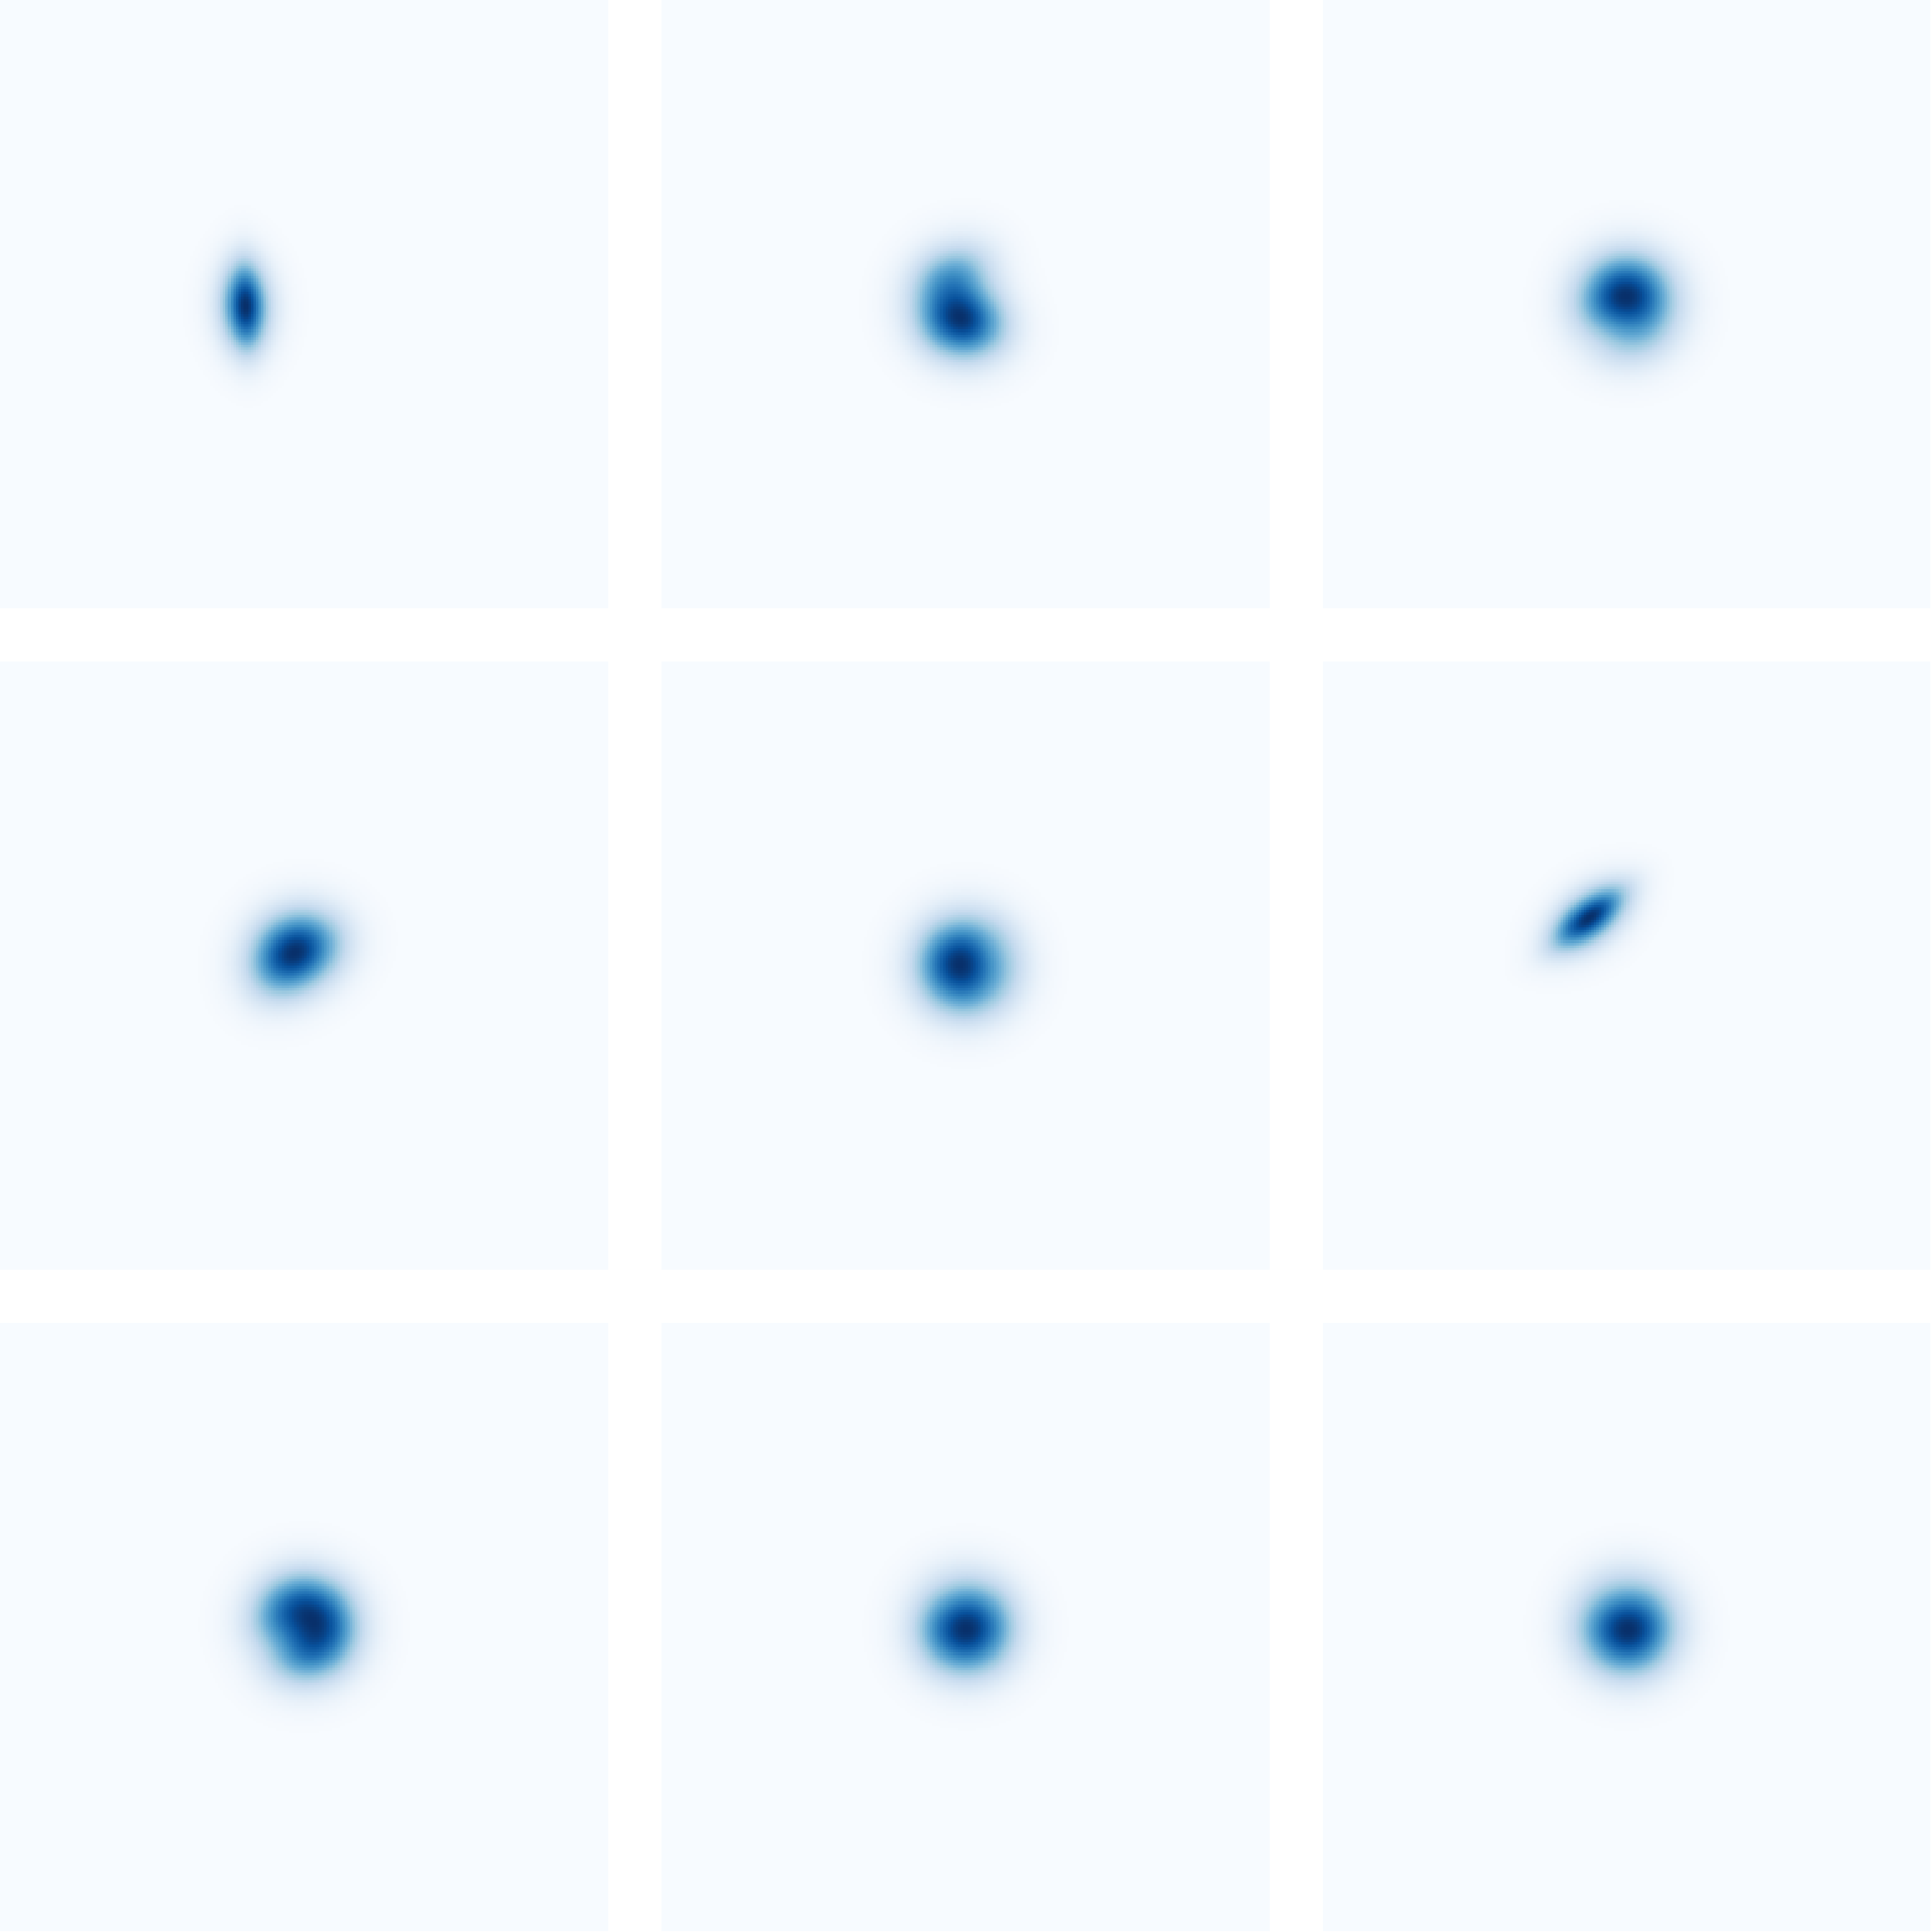
\includegraphics[width=\columnwidth]{pPb_-1p0}}
    \only<2>{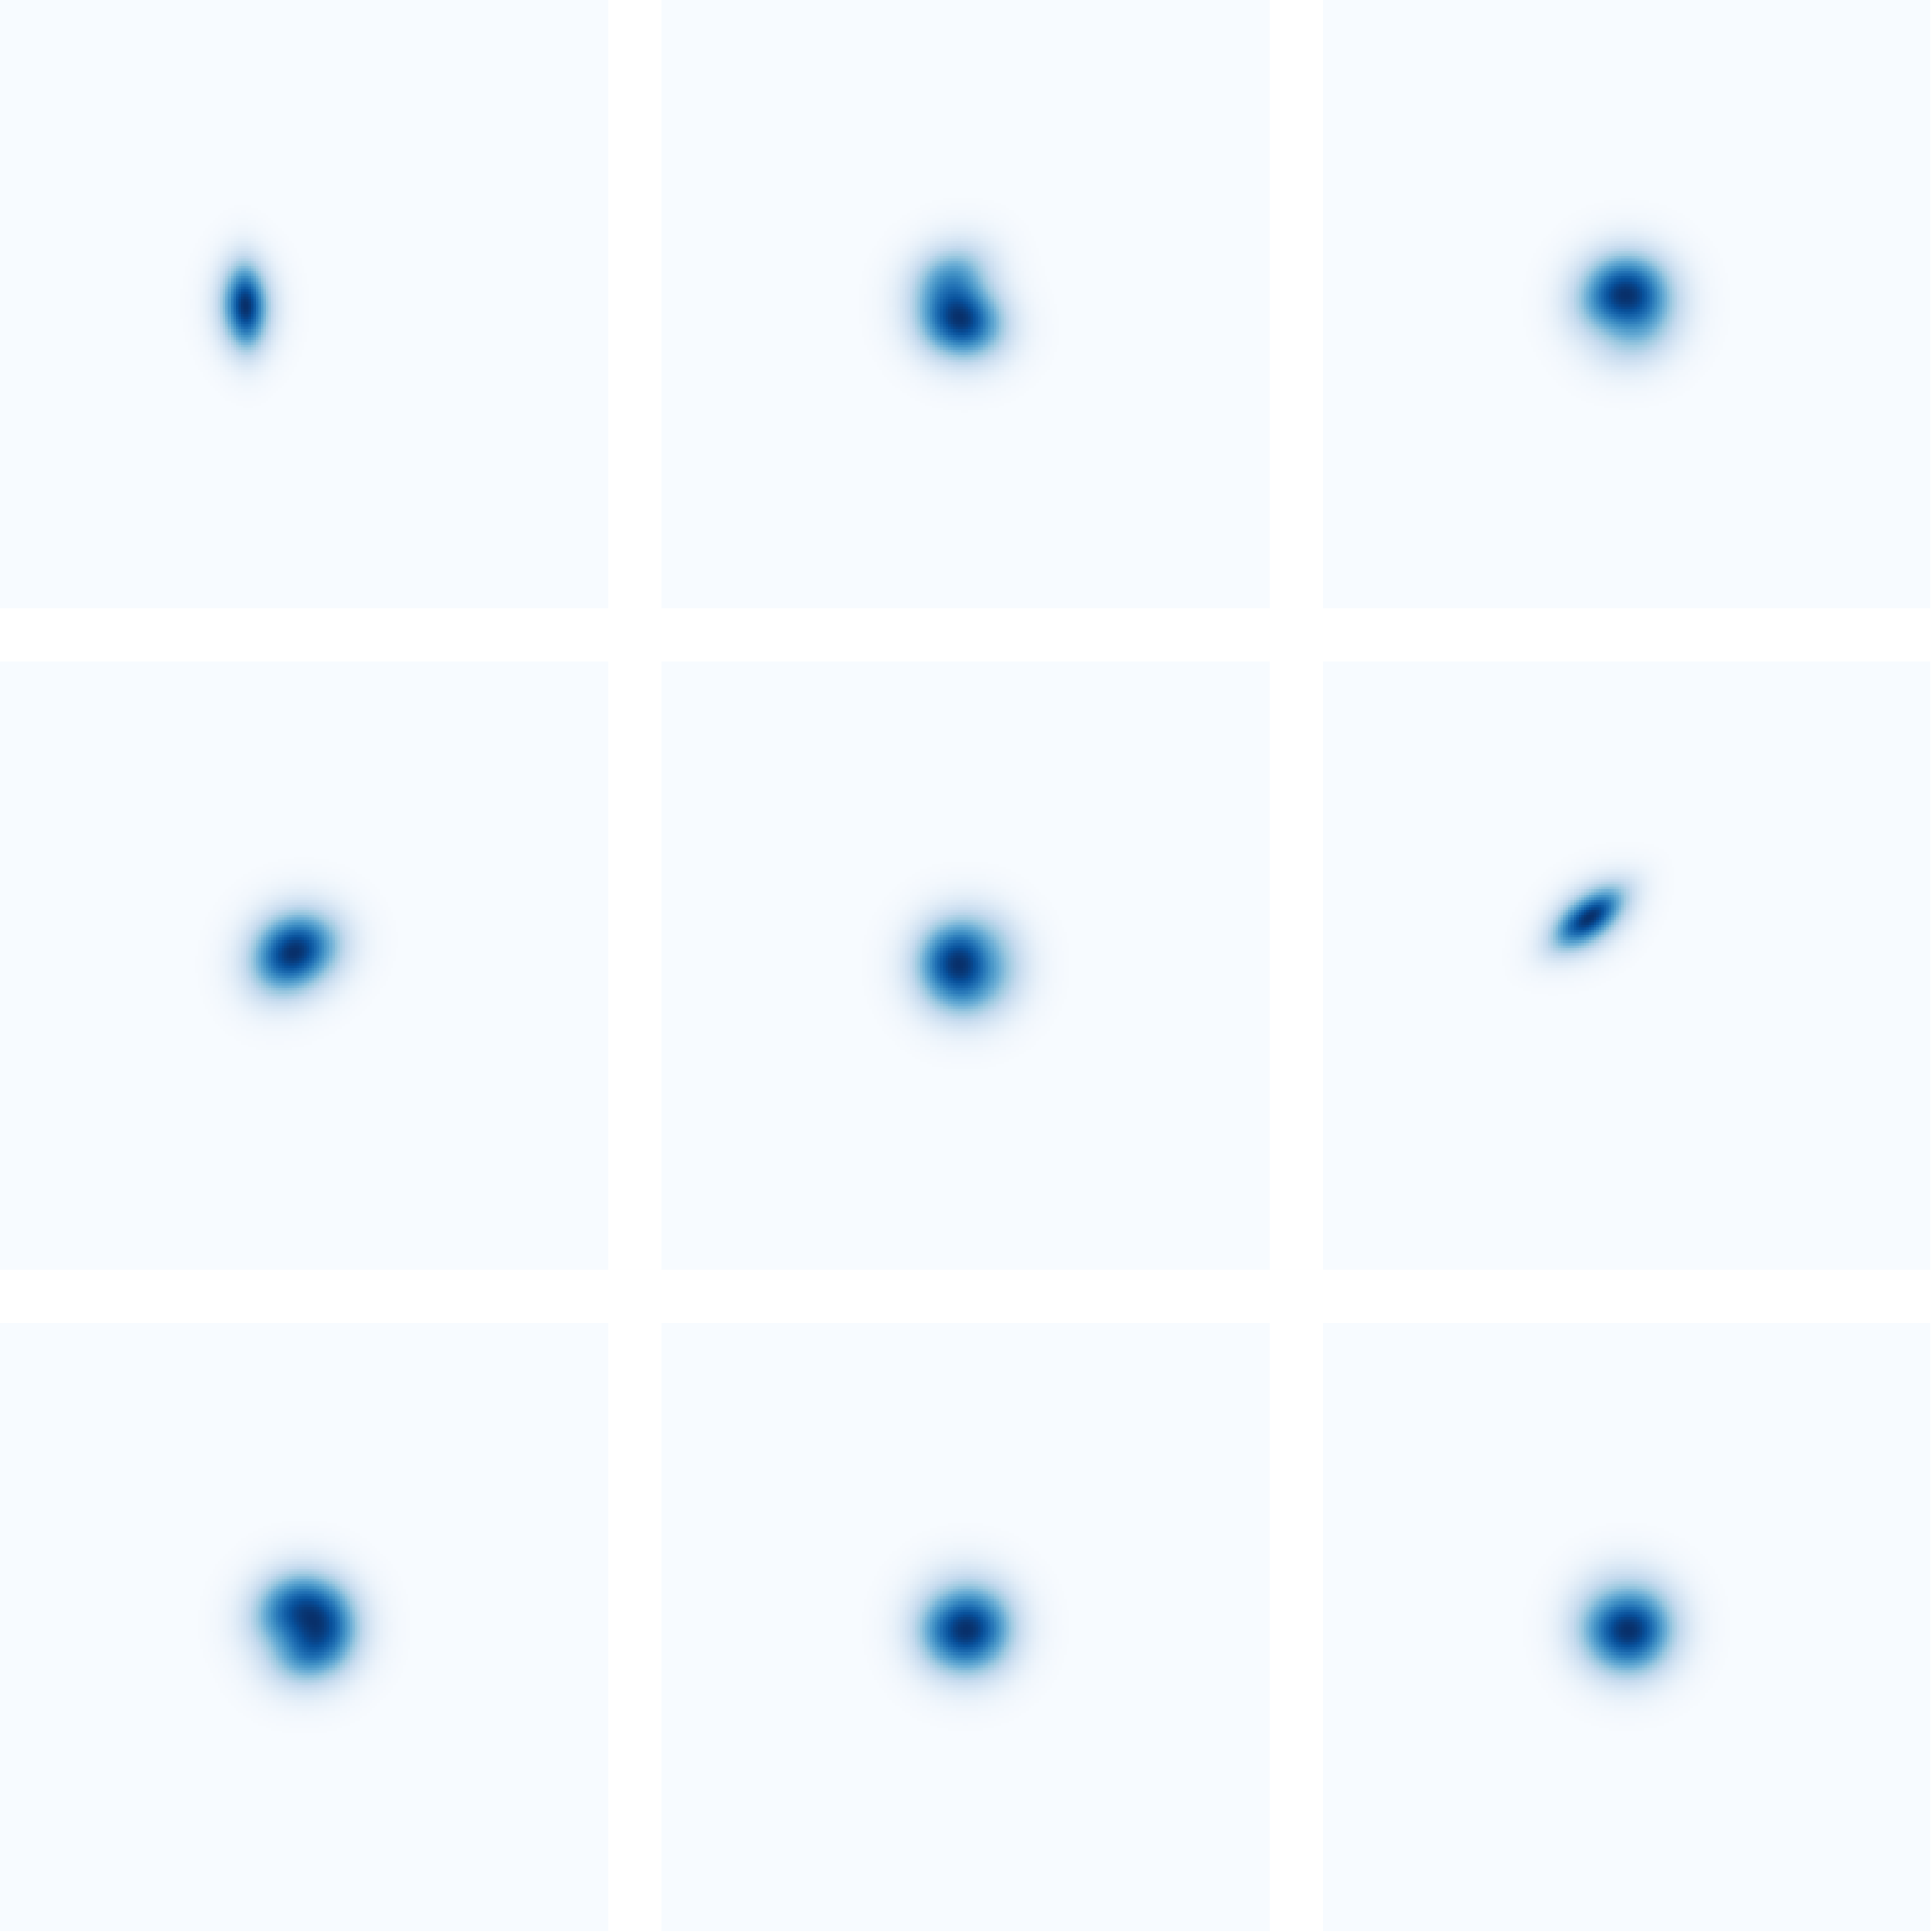
\includegraphics[width=\columnwidth]{pPb_-0p8}}
    \only<3>{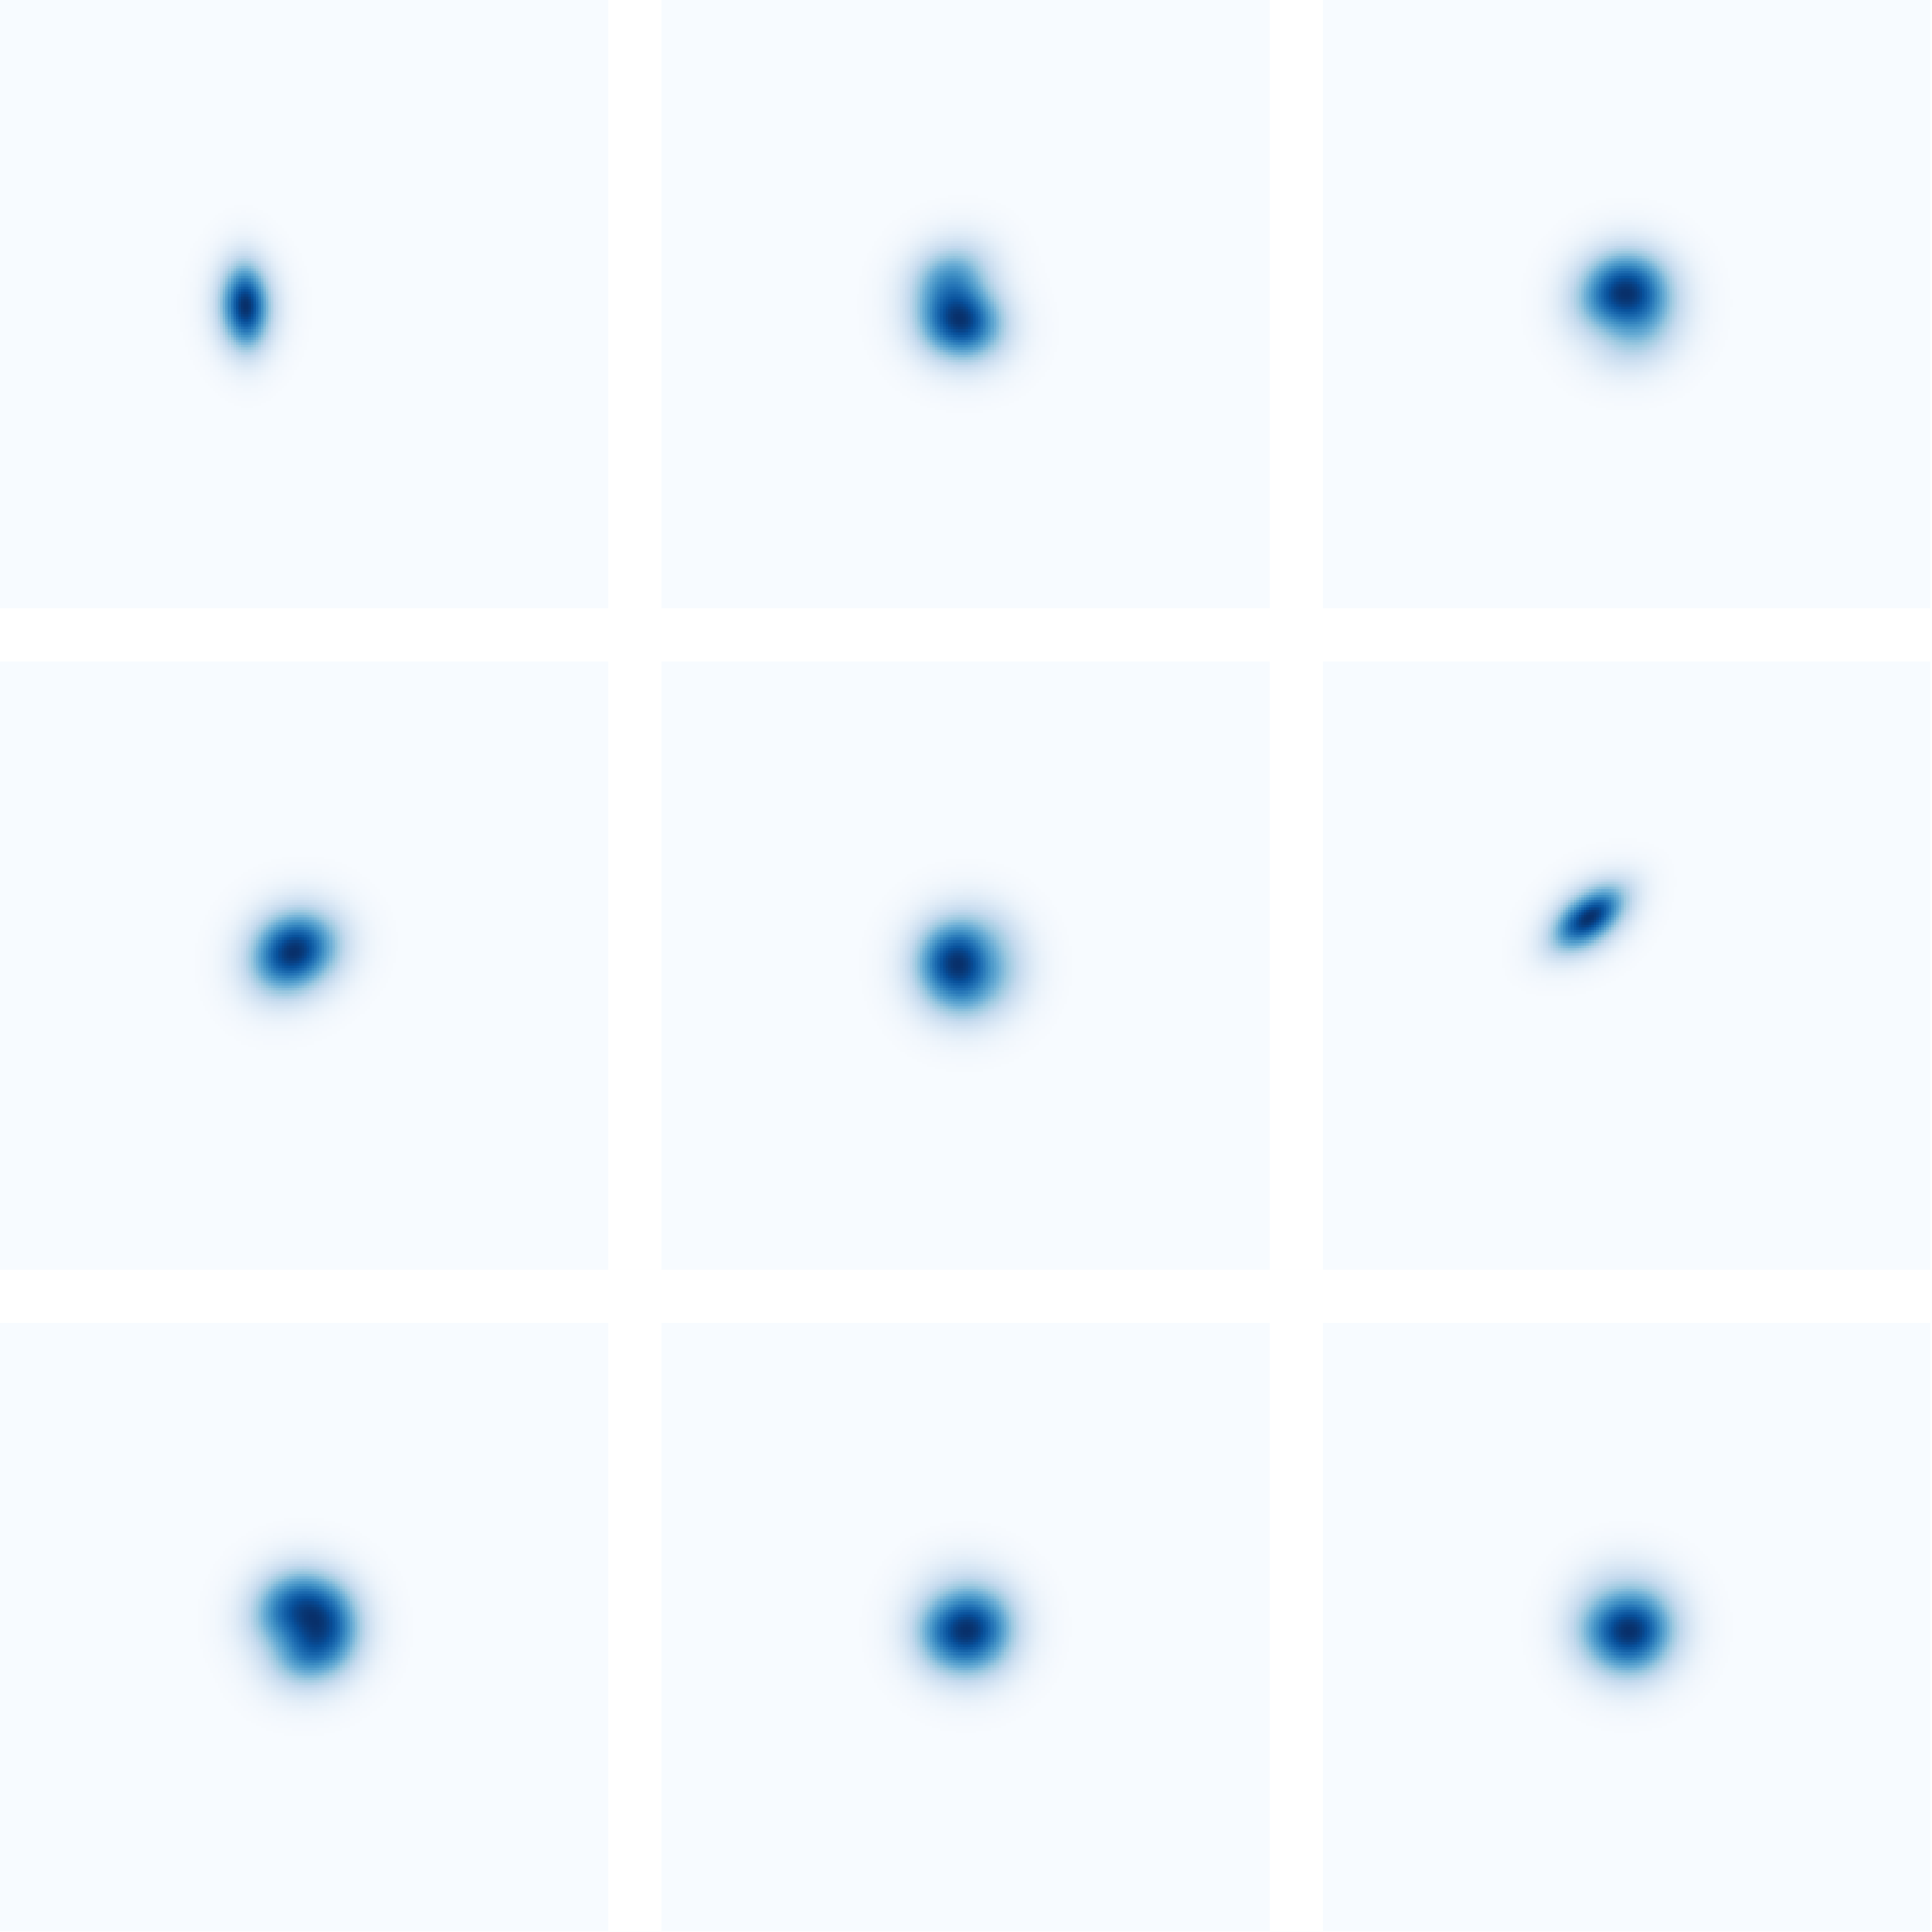
\includegraphics[width=\columnwidth]{pPb_-0p6}}
    \only<4>{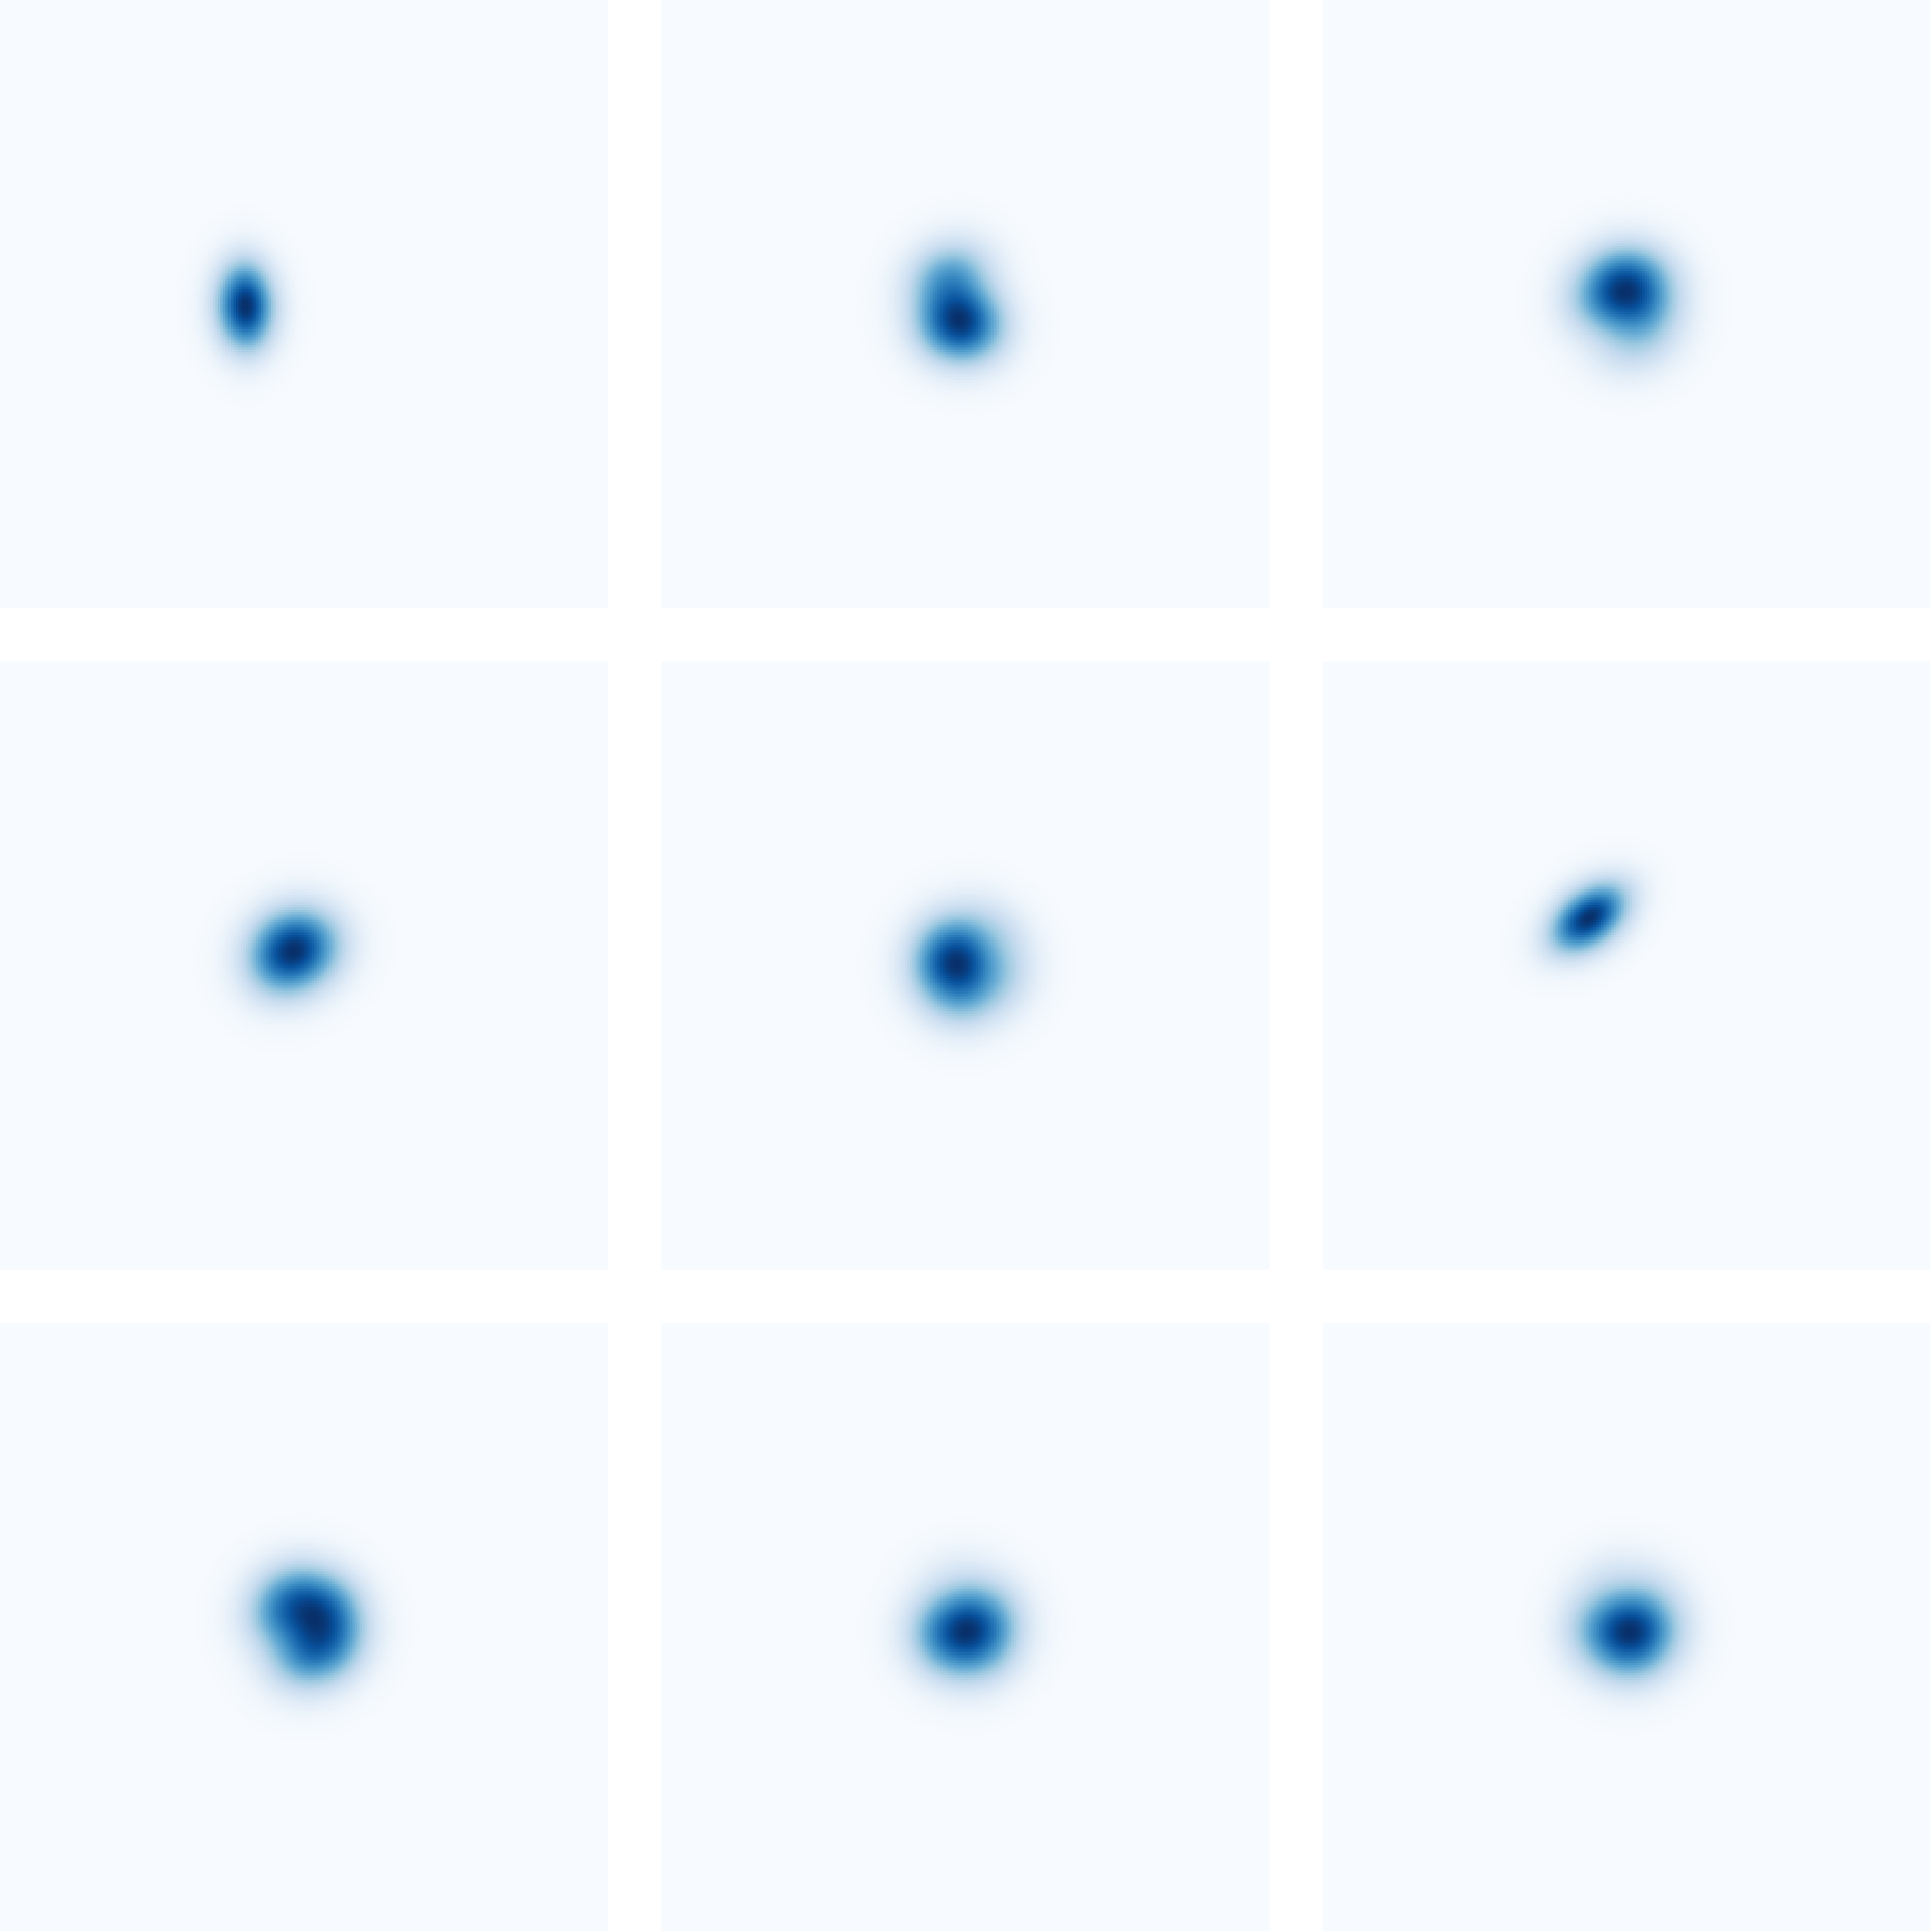
\includegraphics[width=\columnwidth]{pPb_-0p4}}
    \only<5>{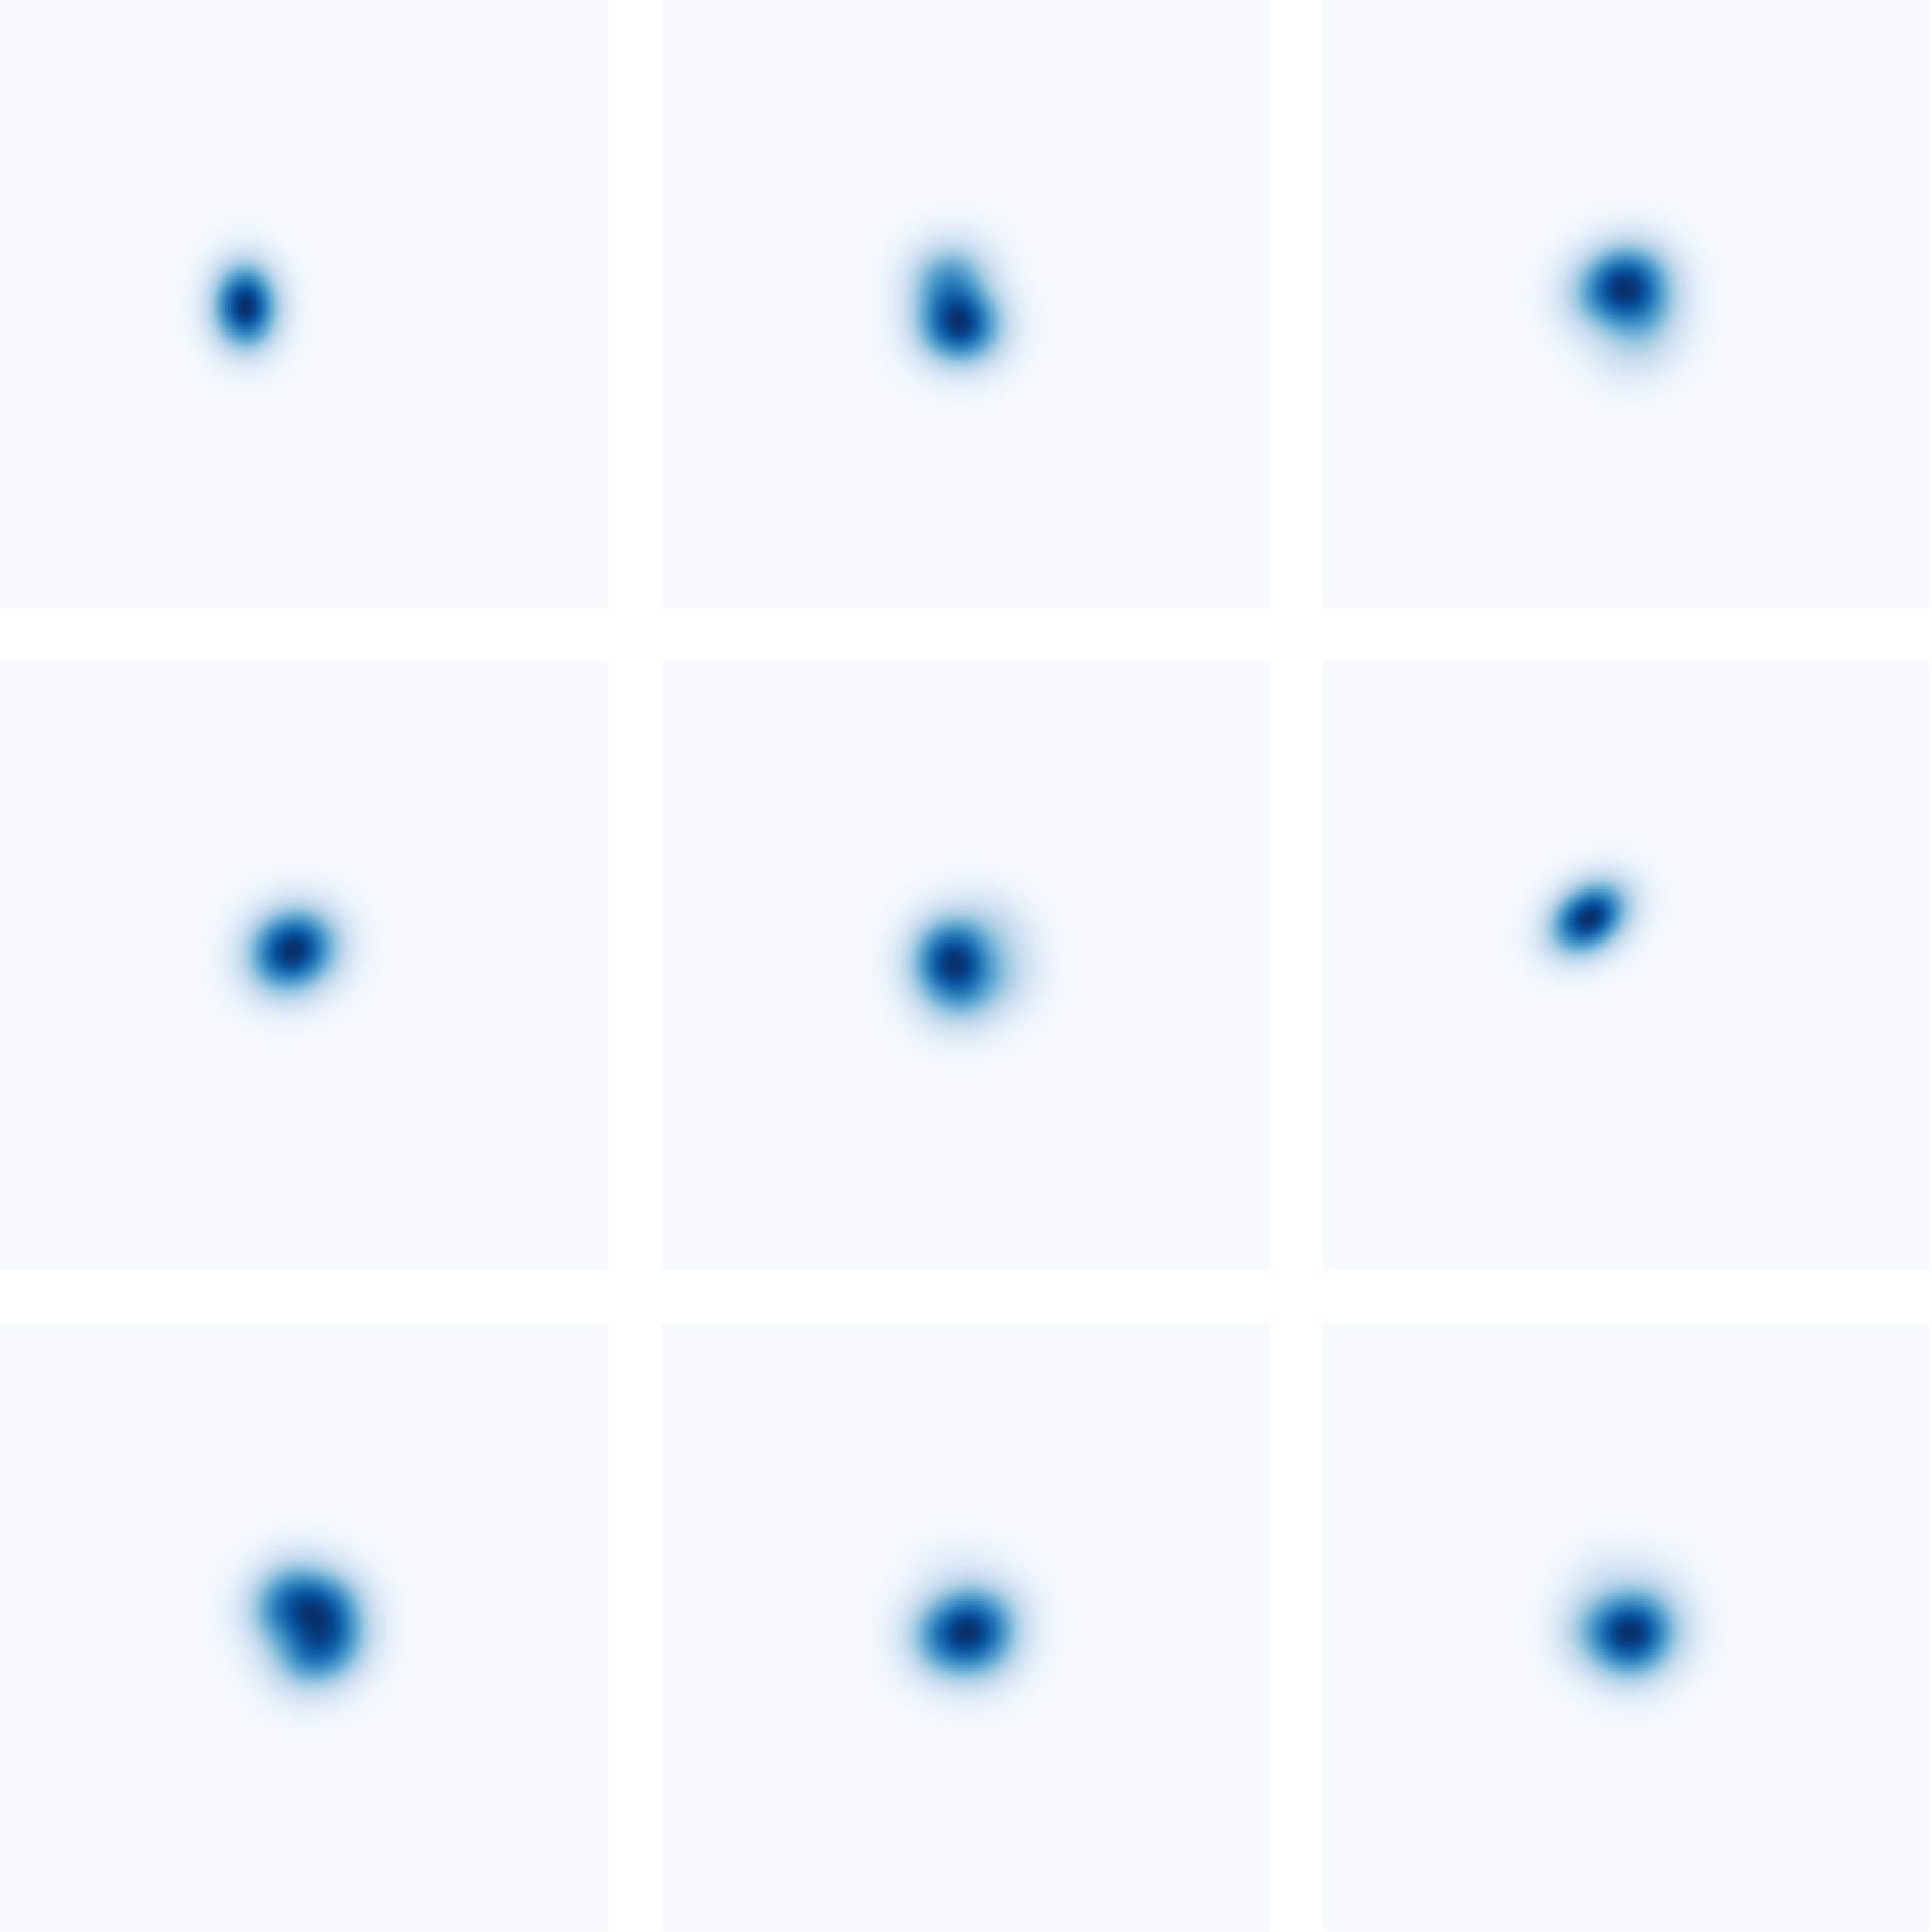
\includegraphics[width=\columnwidth]{pPb_-0p2}}
    \only<6>{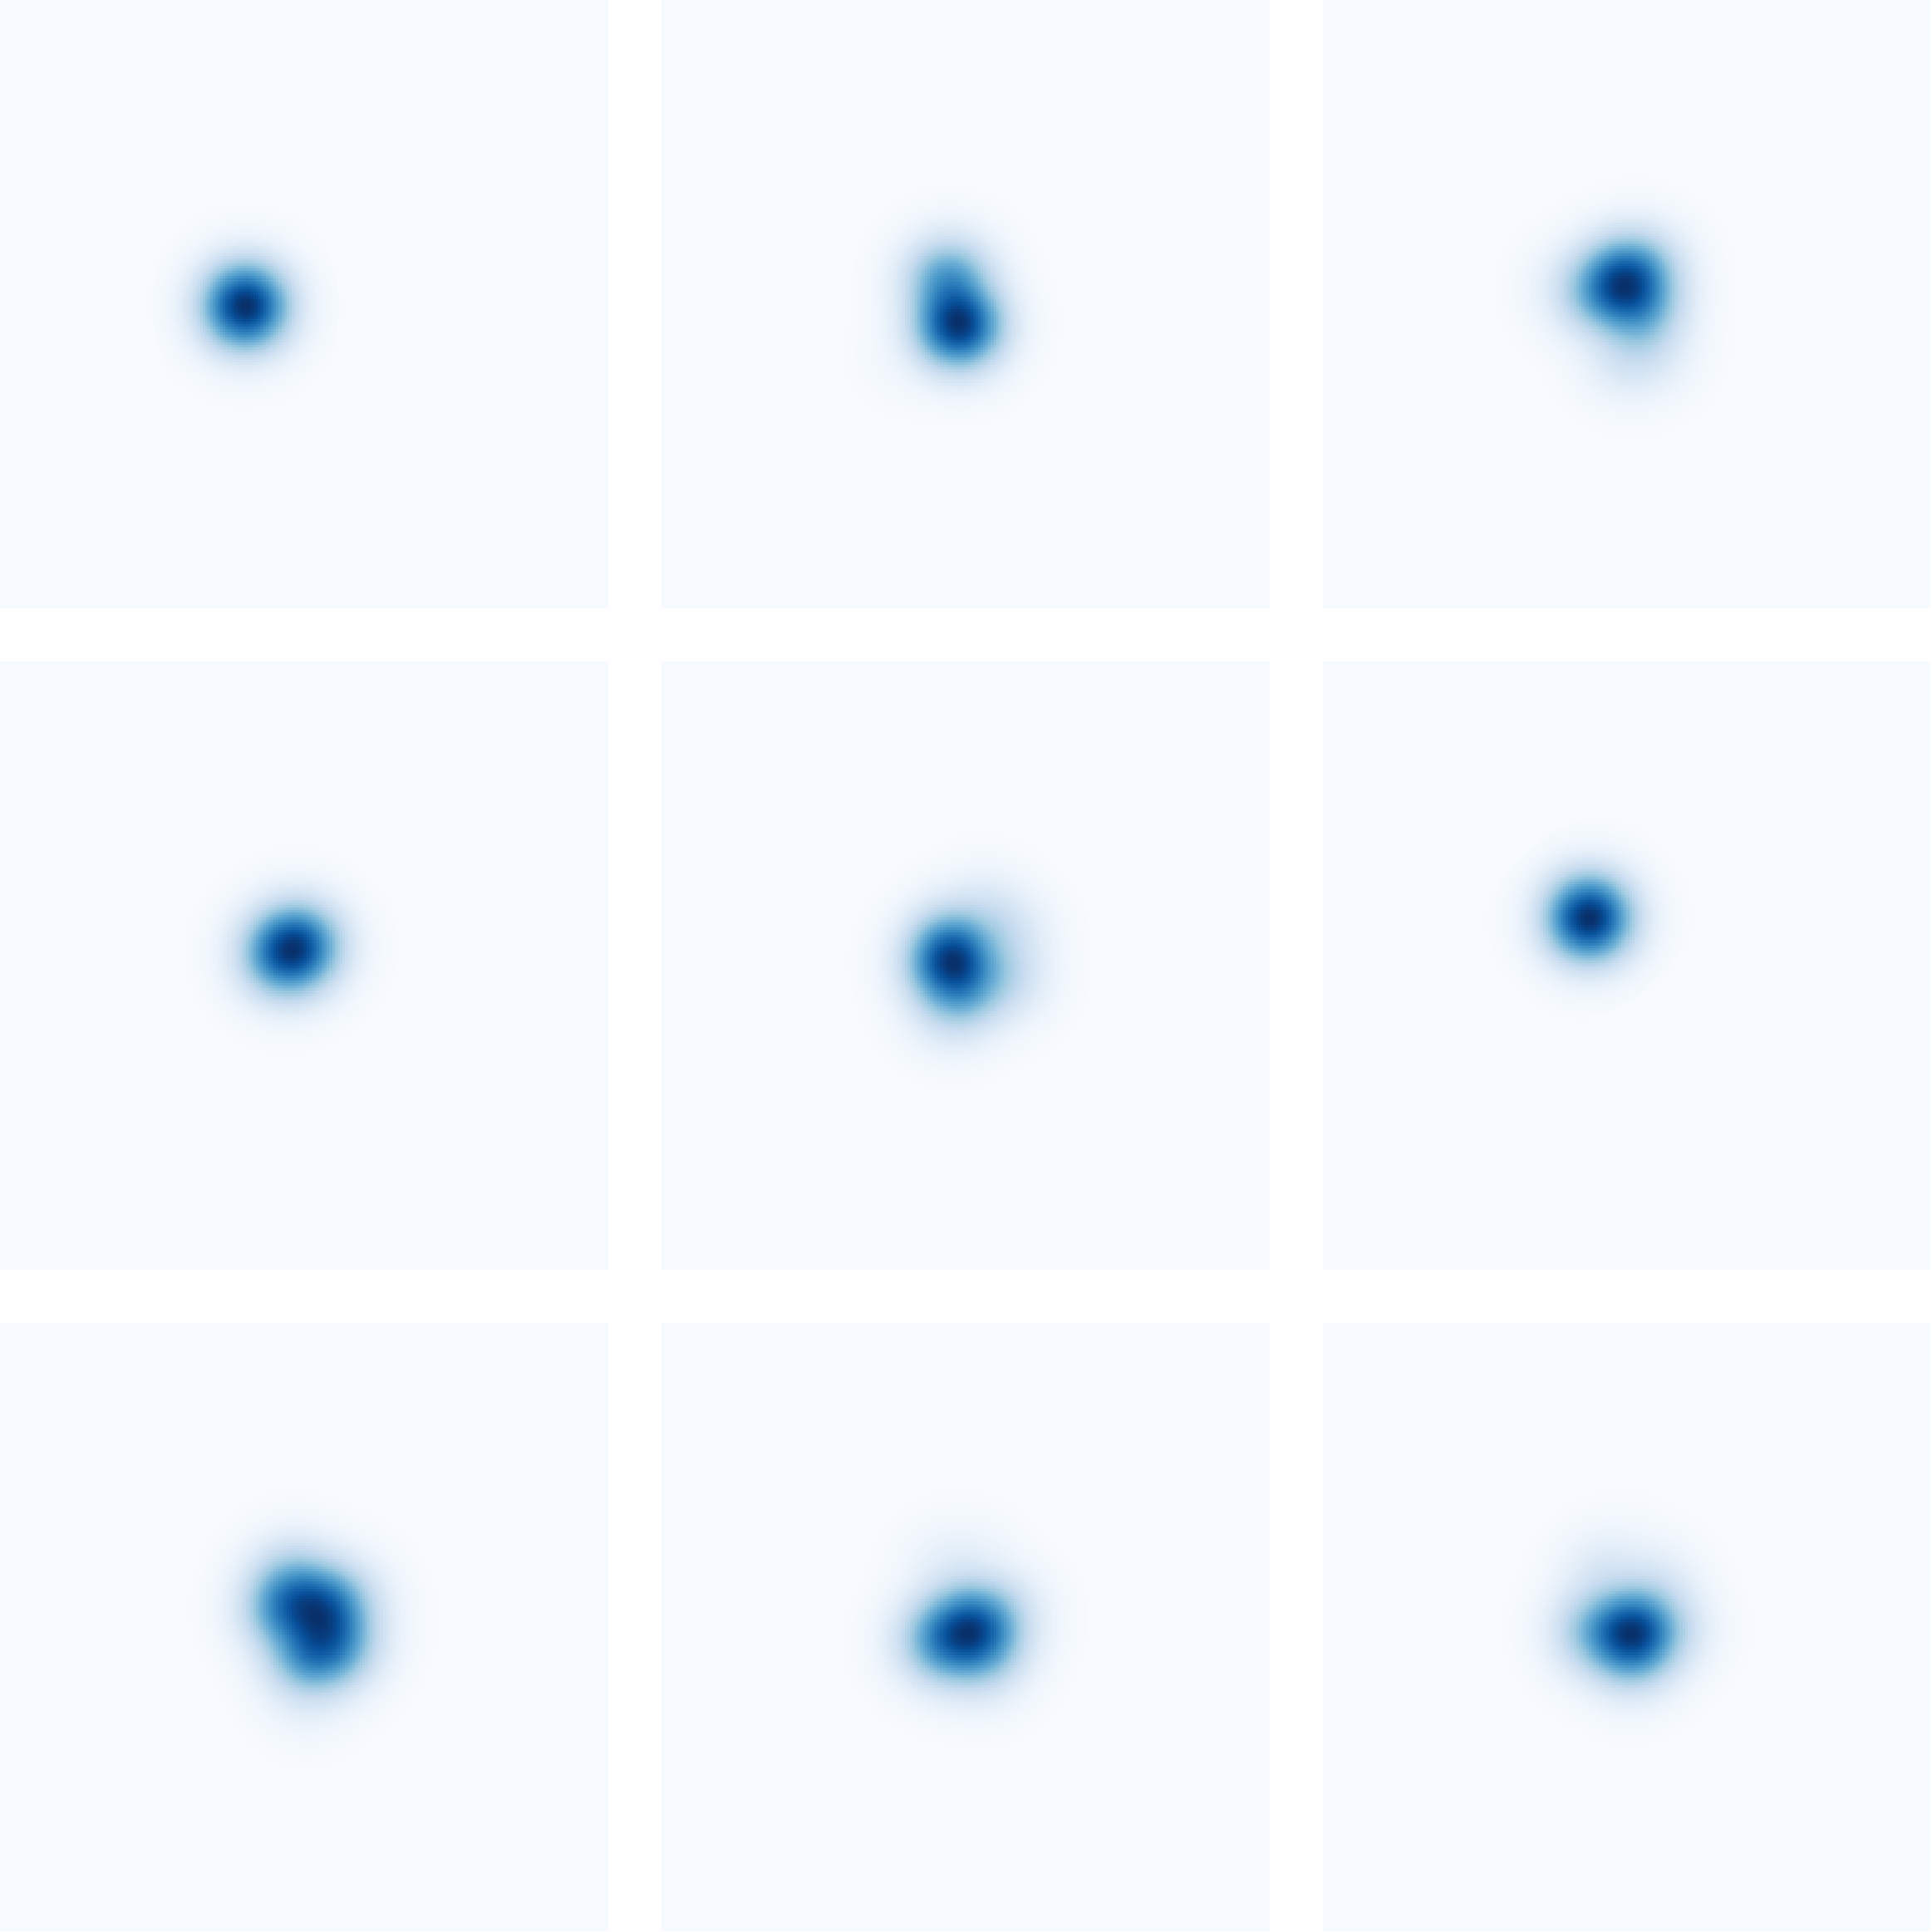
\includegraphics[width=\columnwidth]{pPb_0p0}}
    \only<7>{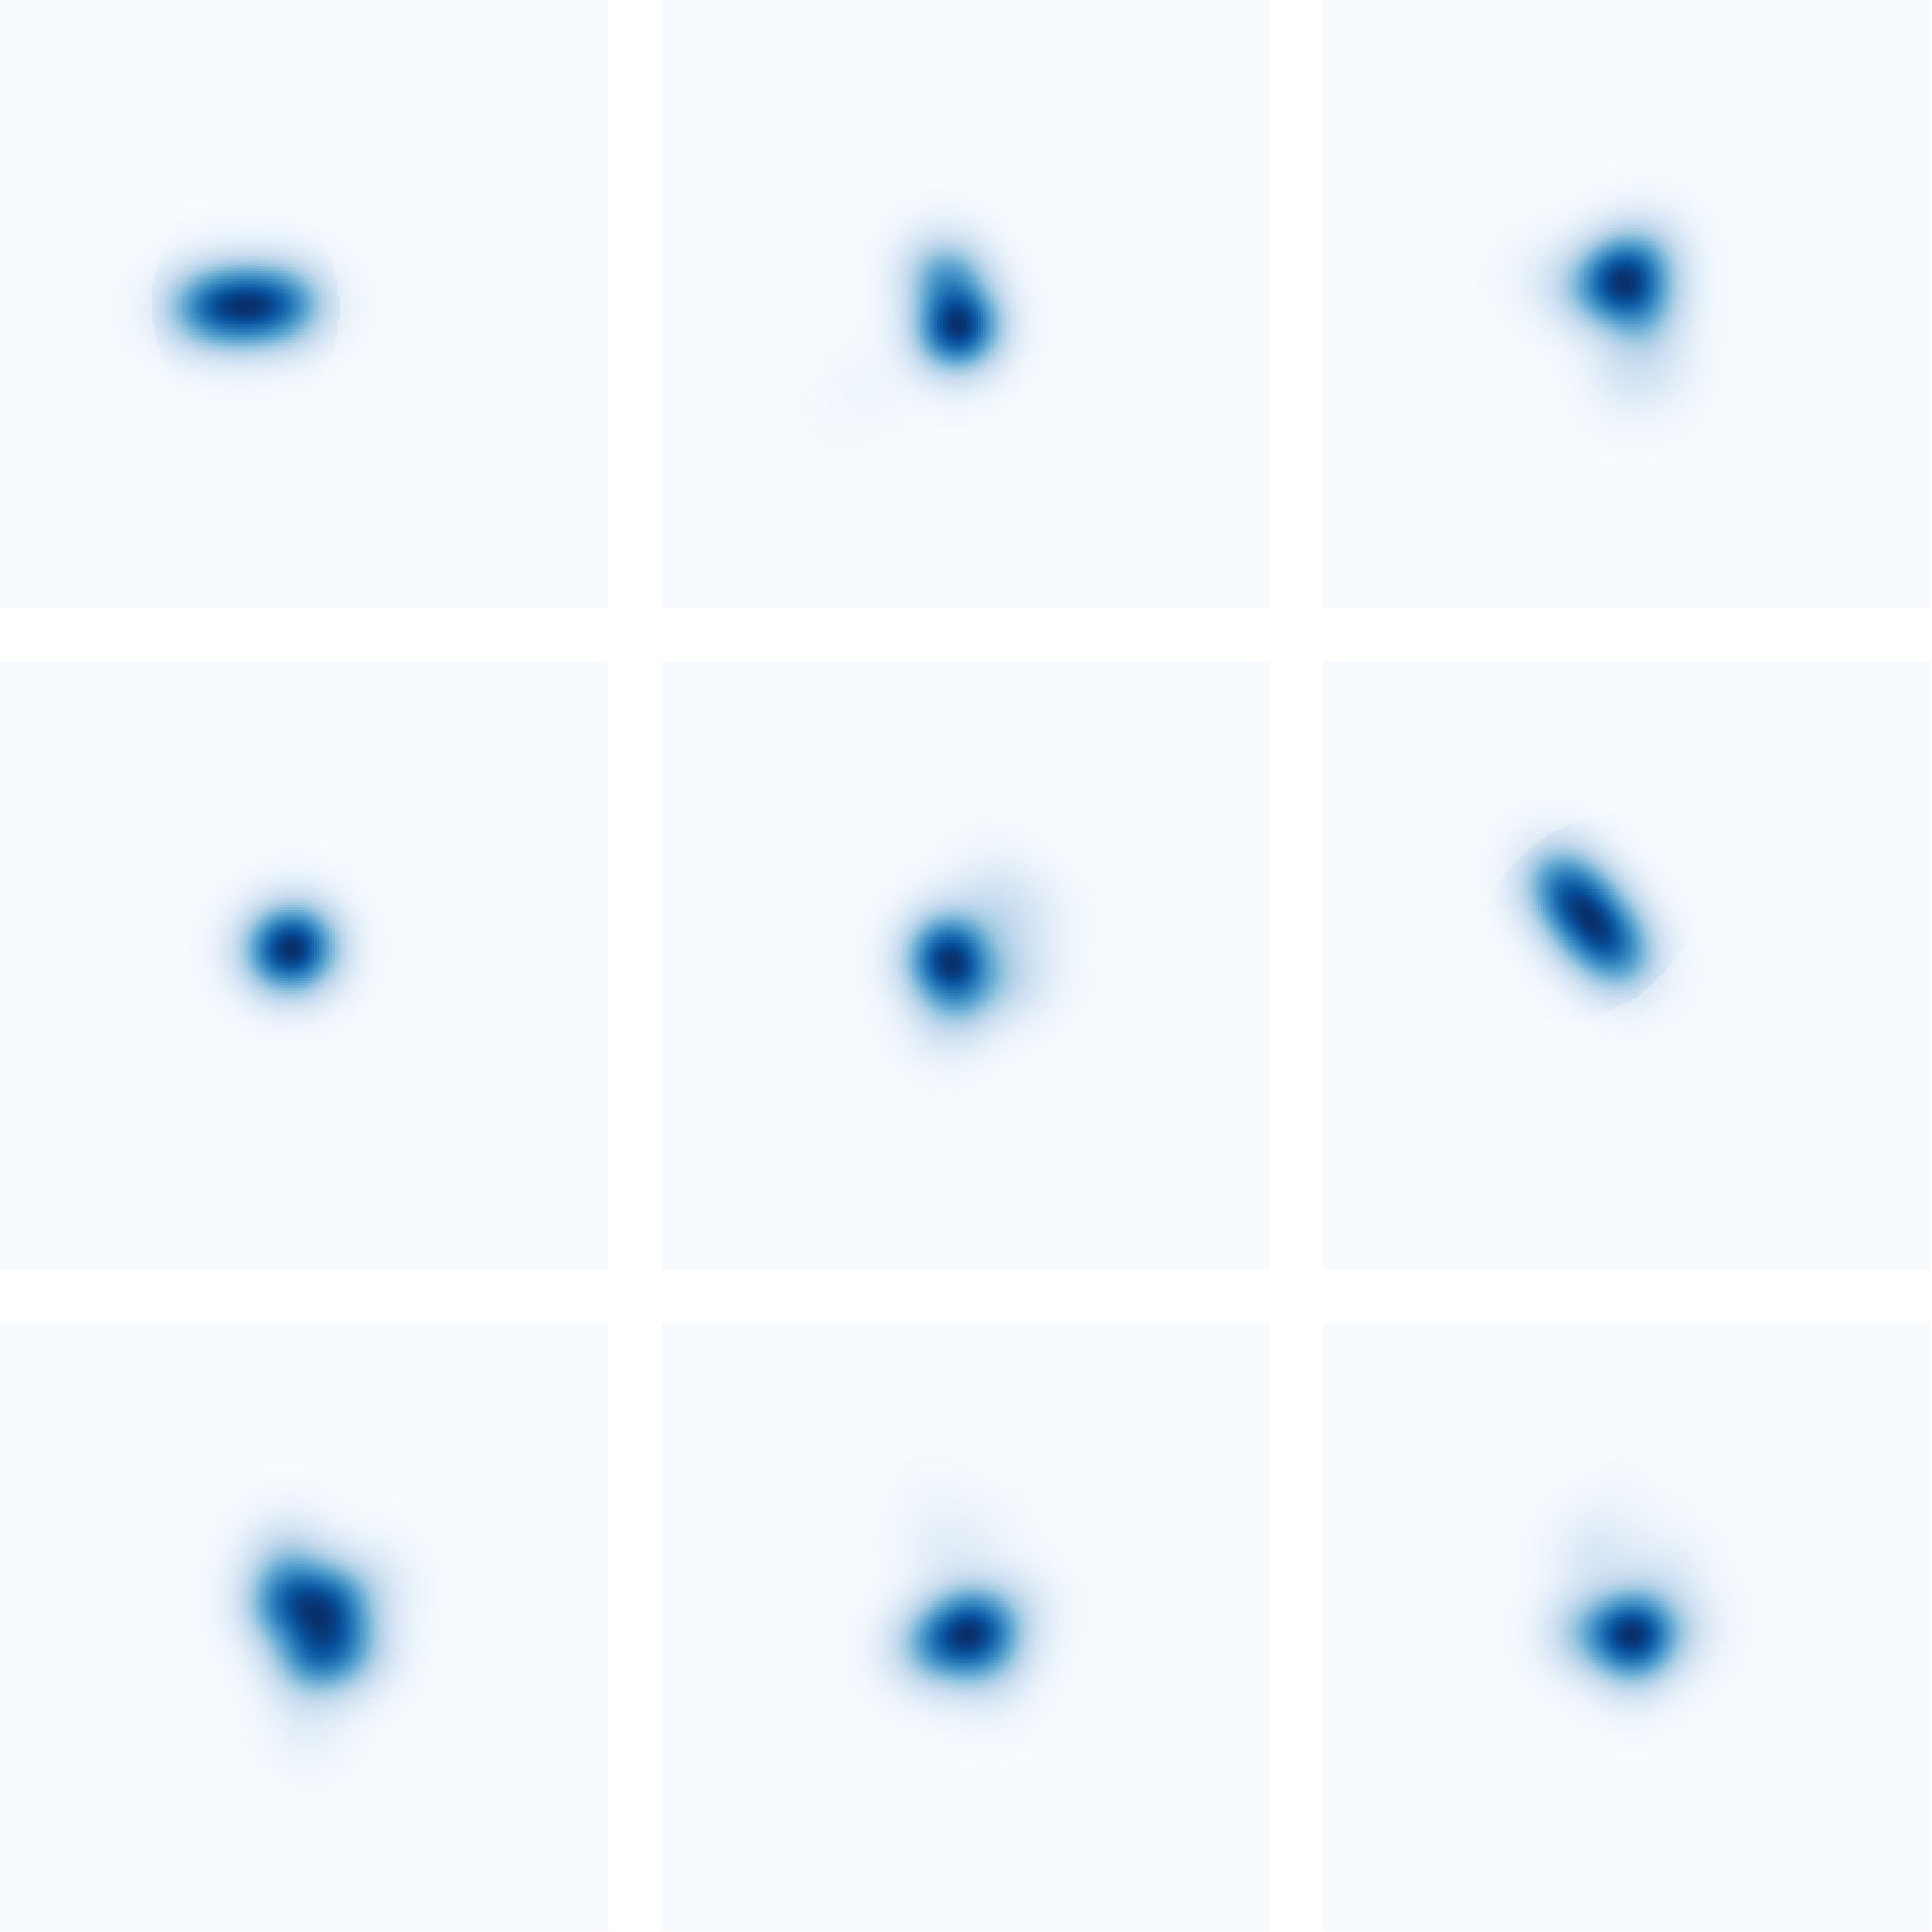
\includegraphics[width=\columnwidth]{pPb_0p2}}
    \only<8>{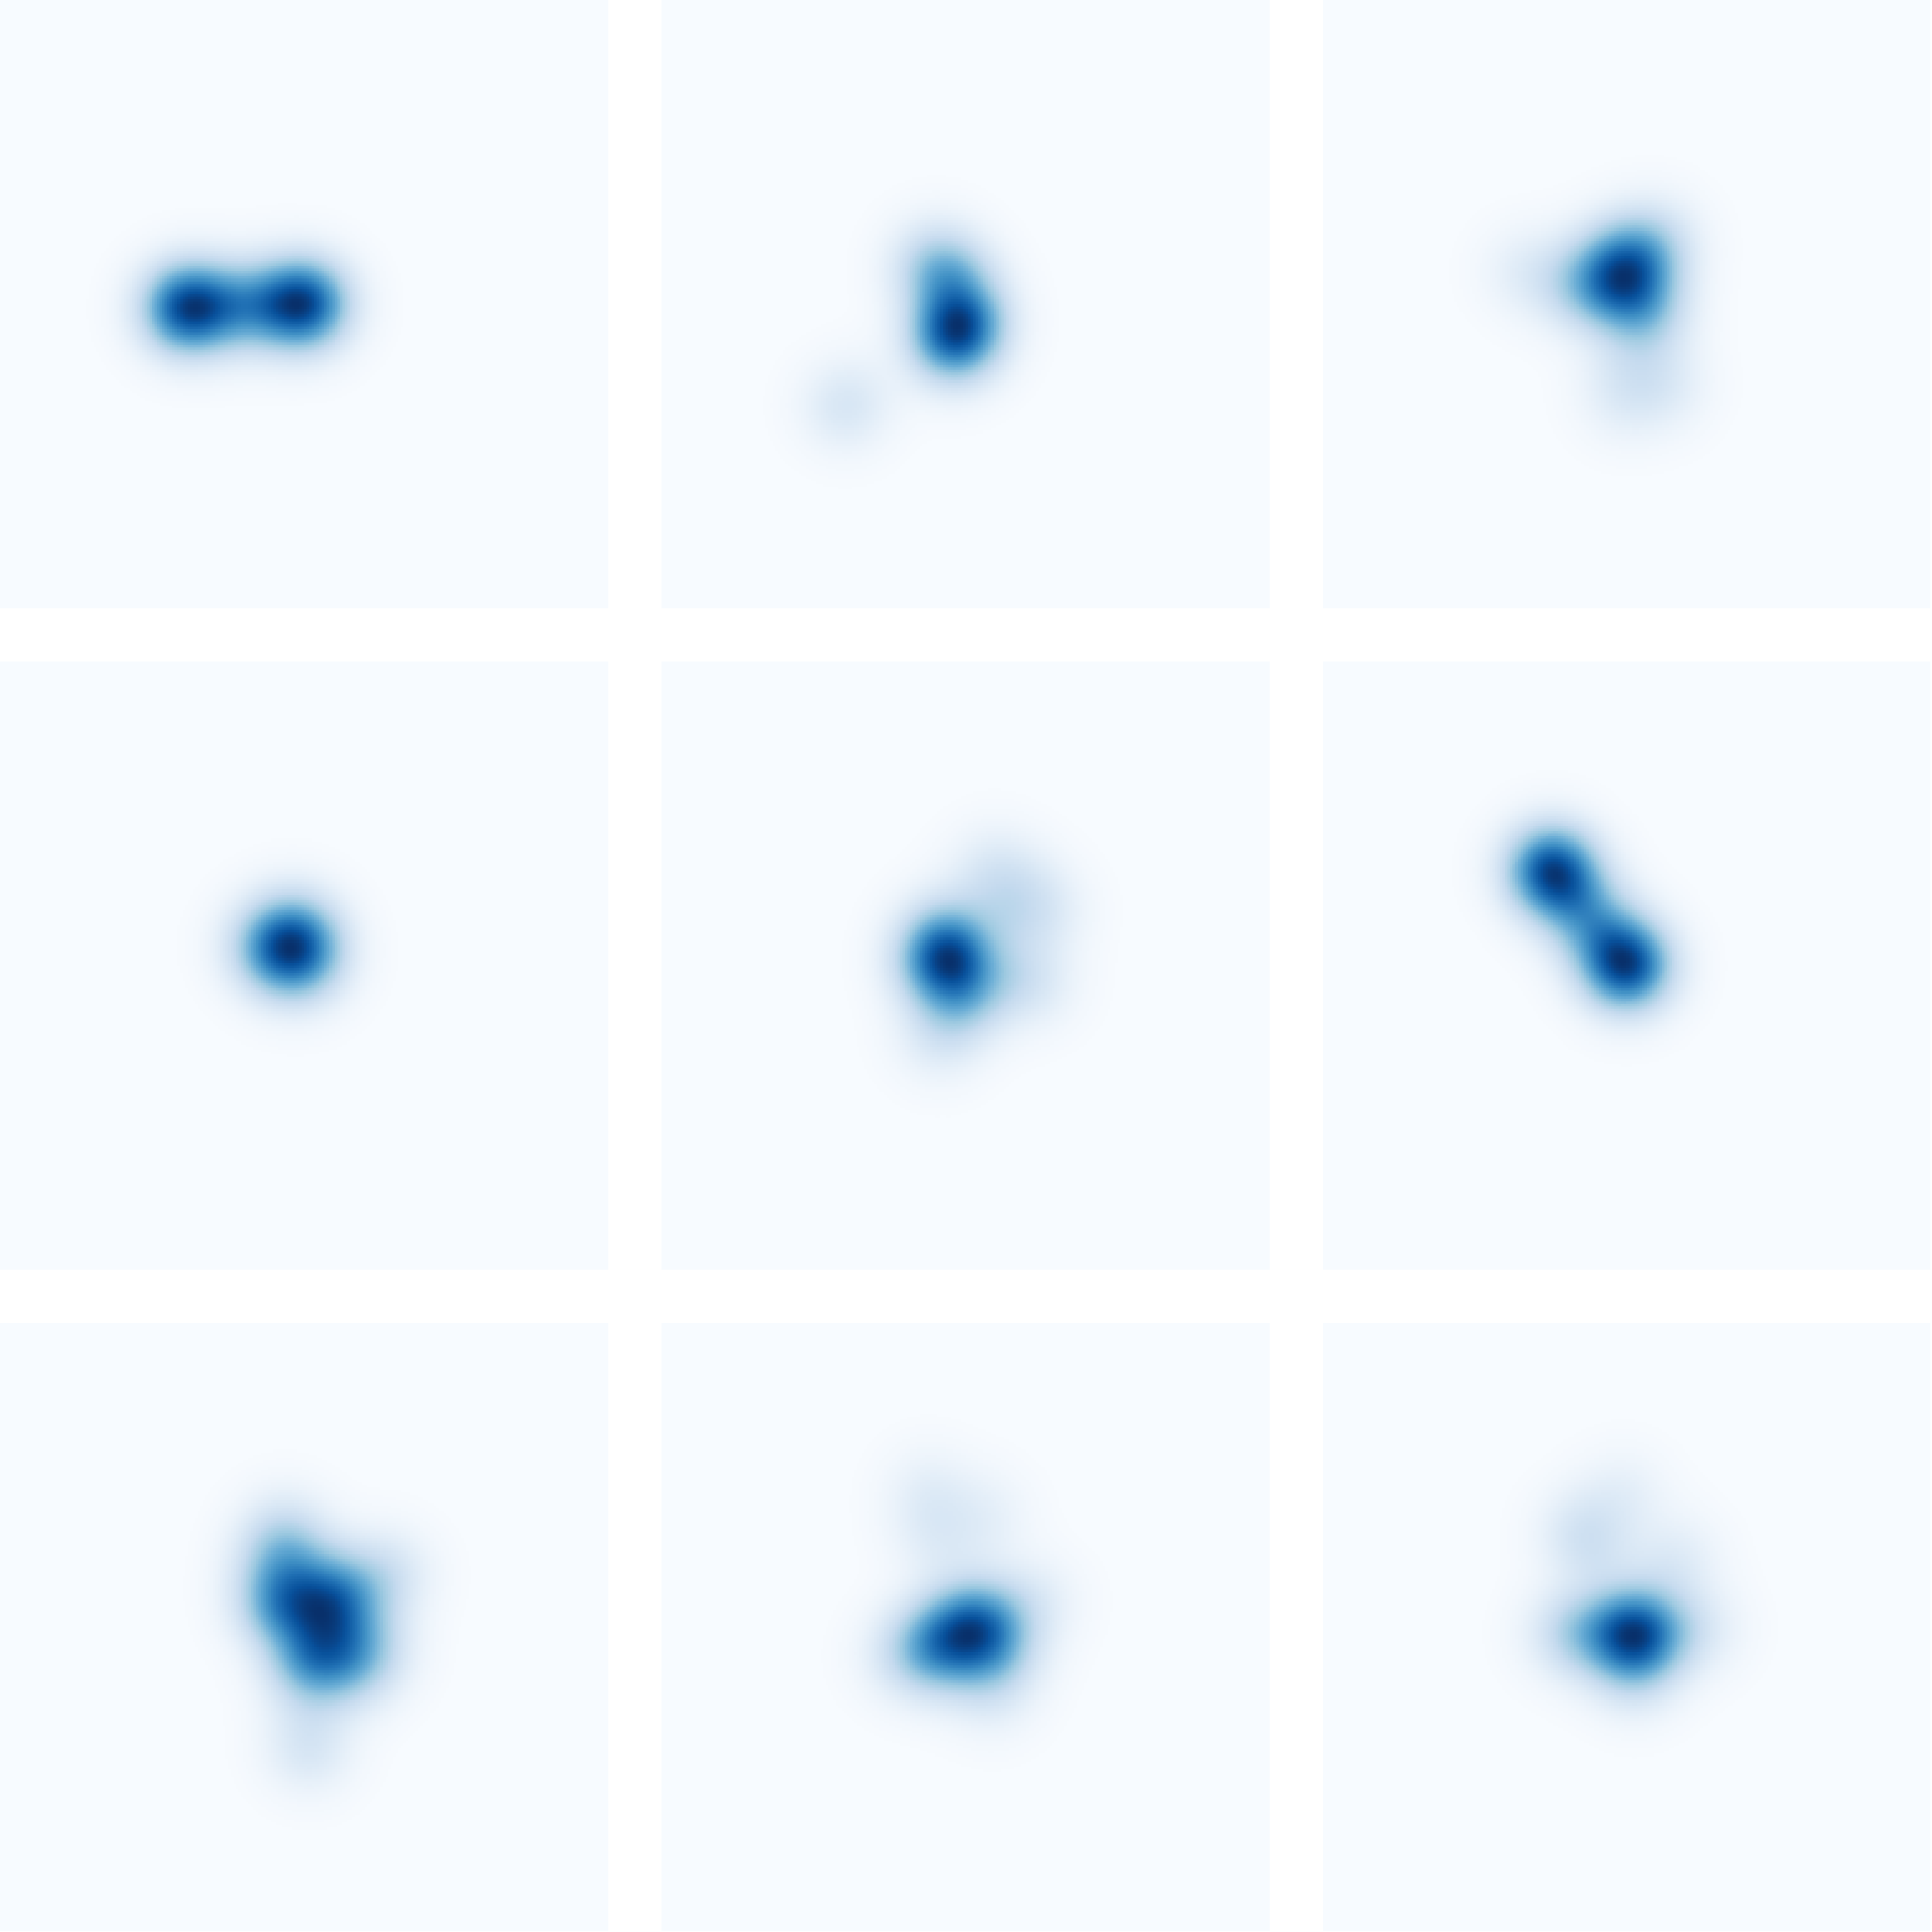
\includegraphics[width=\columnwidth]{pPb_0p4}}
    \only<9>{\includegraphics[width=\columnwidth]{pPb_0p6}}
    \only<10>{\includegraphics[width=\columnwidth]{pPb_0p8}}
    \only<11>{\includegraphics[width=\columnwidth]{pPb_1p0}}
  \end{textblock*}
  
 \end{column}
 
 \begin{column}{0.5\textwidth}
 
  \begin{textblock*}{\linewidth}(0 cm, -3.25 cm)
    \centering d+Au @ 200 GeV
  \end{textblock*}
 
  \begin{textblock*}{\columnwidth}(0 cm, -2.5 cm)
    \centering 
    \only<1>{\includegraphics[width=\columnwidth]{\dAu{dAu_-1p0}}}
    \only<2>{\includegraphics[width=\columnwidth]{\dAu{dAu_-0p8}}}
    \only<3>{\includegraphics[width=\columnwidth]{\dAu{dAu_-0p6}}}
    \only<4>{\includegraphics[width=\columnwidth]{\dAu{dAu_-0p4}}}
    \only<5>{\includegraphics[width=\columnwidth]{\dAu{dAu_-0p2}}}
    \only<6>{\includegraphics[width=\columnwidth]{\dAu{dAu_0p0}}}
    \only<7>{\includegraphics[width=\columnwidth]{\dAu{dAu_0p2}}}
    \only<8>{\includegraphics[width=\columnwidth]{\dAu{dAu_0p4}}}
    \only<9>{\includegraphics[width=\columnwidth]{\dAu{dAu_0p6}}}
    \only<10>{\includegraphics[width=\columnwidth]{\dAu{dAu_0p8}}}
    \only<11>{\includegraphics[width=\columnwidth]{\dAu{dAu_1p0}}}
  \end{textblock*}
  
 \end{column}

\end{columns}

\begin{textblock*}{\linewidth}(0 cm, 3.7 cm)
  \centering
  \begin{tikzpicture}
    \draw[thick,<->] (0,0) -- (10,0);
    \foreach \x in {2.5,5,7.5} \draw[thick] (\x cm,2pt) -- (\x cm,-2pt);
    \draw (0,0) node[below=3pt] {$ -\infty $} node[above=3pt] {min};
    \draw (2.5,0) node[below=3pt] {$ -1 $} node[above=3pt] {harmonic};
    \draw (5,0) node[below=3pt] {$ 0 $} node[above=3pt] {geometric};
    \draw (7.5,0) node[below=3pt] {$ 1 $} node[above=3pt] {arithmetic};
    \draw (10,0) node[below=3pt] {$ \infty $} node[above=3pt] {max};
    \only<1>{\draw[black,fill=black] (2.5,0) circle (0.1 cm);}
    \only<2>{\draw[black,fill=black] (3,0) circle (0.1 cm);}
    \only<3>{\draw[black,fill=black] (3.5,0) circle (0.1 cm);}
    \only<4>{\draw[black,fill=black] (4,0) circle (0.1 cm);}
    \only<5>{\draw[black,fill=black] (4.5,0) circle (0.1 cm);}
    \only<6>{\draw[black,fill=black] (5,0) circle (0.1 cm);}
    \only<7>{\draw[black,fill=black] (5.5,0) circle (0.1 cm);}
    \only<8>{\draw[black,fill=black] (6,0) circle (0.1 cm);}
    \only<9>{\draw[black,fill=black] (6.5,0) circle (0.1 cm);}
    \only<10>{\draw[black,fill=black] (7,0) circle (0.1 cm);}
    \only<11>{\draw[black,fill=black] (7.5,0) circle (0.1 cm);}
  \end{tikzpicture}
\end{textblock*}

\begin{textblock*}{1.01\linewidth}(-0.12 cm, -2.85 cm)
  \centering
  \textcolor{gray}{\rule{1.01\linewidth}{0.6 pt}}
\end{textblock*}

\begin{textblock*}{\linewidth}(0 cm, -3.15 cm)
  \centering
  \textcolor{gray}{\rule{0.6 pt}{6.5 cm}}
\end{textblock*}

\end{frame}

%%%%%%%%%%%%%%%%%%
\begin{frame}{Constraining entropy deposition with multiple systems}
 \centering
 \vspace{0.1 in} 
 \only<1>{\includegraphics[width=\textwidth]{rhic_p=0p3}}
 \only<2>{\includegraphics[width=\textwidth]{rhic_p=1}}
\end{frame}

%%%%%%%%%%%%%%%%%%
\begin{frame}{Summary}
\begin{itemize}
 \item Introduce \trento\,, a new parametric model which deposits entropy proportional to the generalized mean of participant matter.
 \item Model can mimic behaviour of well known initial conditions models such as KLN and IP-Glasma.
 \item Preliminary results (no hydro!) indicate that the LHC prefers $p \approx 0$ which closely mimics IP-Glasma scaling. RHIC prefers $p \approx 0.3$.
 \item Model prefers entropy deposition in p+p and p+A collisions which is more eikonal, i.e. localized in p+p overlap region.
 \item Currently working on embedding model in systematic Bayesian analysis to extract QGP medium and initial state properties simultaneously.\\
 \vspace{0.2 in}
 \centering Model available at: \url{https://github.com/Duke-QCD/trento}
\end{itemize}

 
\end{frame}



\end{document}
